\chapter{Traffic engineering with SR}
\label{chapter:te}

\section*{Introduction}

In this chapter we propose a column generation algorithm for solving the traffic engineering (TE) problem 
on a network using segment routing. The traffic engineering problem consists of routing a set of demands over the 
network whilst minimizing congestion. Routing traffic between a source
and a destination along shortest paths allows for no flexibility regarding the way this traffic is send which may lead to a suboptimal 
usage of the network infrastructure.
Consider the four router network show in Figure \ref{fig:te-example}. Suppose that we want to route three demands on this network, all from
\node{a} to \node{b}. Assuming unit IGP weights, all those demands will traverse the link $(\node{a}, \node{d})$. In contrast, we could
route one of them via \node{b} and the other via \node{c} as shown on the right. This second solution leads to a much more efficient
utilisation of the network. It spreads the traffic thus leading to less congestion. Assuming equal demand volumes, the solution on the right
improves the congestion of the link $(\node{a}, \node{b})$ by $66\%$. This is a very small example and even here we can already see the limitations of shortest path routing for TE. 

\begin{figure}[H]
\begin{center}
\begin{tabular}{ccc}
\begin{tikzpicture}[scale=1.2]
%\node[draw, circle] (a) at (0, 0) {\tiny \texttt{a}};

\node[scale=0.15] (a) at (0, 0)     {\router{a}{router}};
\node[scale=0.15] (b) at (1, 1)    {\router{b}{router}};
\node[scale=0.15] (c) at (1, -1)     {\router{c}{router}};
\node[scale=0.15] (d) at (2, -0)    {\router{d}{router}};

\draw[line width=2] (a) edge[above, sloped] node[black,font=\bfseries] {\footnotesize \texttt{}} (b);
\draw[line width=2] (a) edge[above, sloped] node[black,font=\bfseries] {\footnotesize \texttt{}} (c);
\draw[line width=2] (a) edge[above, sloped] node[black,font=\bfseries] {\footnotesize \texttt{}} (d);
\draw[line width=2] (b) edge[above, sloped] node[black,font=\bfseries] {\footnotesize \texttt{}} (d);
\draw[line width=2] (c) edge[above, sloped] node[black,font=\bfseries] {\footnotesize \texttt{}} (d);

\draw[cyan, line width=2, ->] plot [smooth] coordinates { (0.5, 0.2) (1.5, 0.2) };
\draw[orange, line width=2, ->] plot [smooth] coordinates { (0.5, 0) (1.5, 0) };
\draw[darkgreen, line width=2, ->] plot [smooth] coordinates { (0.5, -0.2) (1.5, -0.2) };

\end{tikzpicture}

&

$\quad$

&

\begin{tikzpicture}[scale=1.2]
%\node[draw, circle] (a) at (0, 0) {\tiny \texttt{a}};

\node[scale=0.15] (a) at (0, 0)     {\router{a}{router}};
\node[scale=0.15] (b) at (1, 1)    {\router{b}{router}};
\node[scale=0.15] (c) at (1, -1)     {\router{c}{router}};
\node[scale=0.15] (d) at (2, -0)    {\router{d}{router}};

\draw[line width=2] (a) edge[above, sloped] node[black,font=\bfseries] {\footnotesize \texttt{}} (b);
\draw[line width=2] (a) edge[above, sloped] node[black,font=\bfseries] {\footnotesize \texttt{}} (c);
\draw[line width=2] (a) edge[above, sloped] node[black,font=\bfseries] {\footnotesize \texttt{}} (d);
\draw[line width=2] (b) edge[above, sloped] node[black,font=\bfseries] {\footnotesize \texttt{}} (d);
\draw[line width=2] (c) edge[above, sloped] node[black,font=\bfseries] {\footnotesize \texttt{}} (d);

\draw[cyan, line width=2, ->] plot [smooth] coordinates { (0, 0.5) (0.3, 1) (1, 1.5) (1.8, 1) (2, 0.5) };
\draw[orange, line width=2, ->] plot [smooth] coordinates { (0.5, 0) (1.5, 0) };
\draw[darkgreen, line width=2, ->] plot [smooth] coordinates { (0, -0.5) (0.3, -1) (1, -1.5) (1.8, -1) (2, -0.5) };

\end{tikzpicture}
\end{tabular}
\end{center}
\caption{Small example where shortest path routing is not ideal for TE.}
\label{fig:te-example}
\end{figure}

Attempts at solving the TE problem can be categorized into two main categories. On one hand we could improve the way a set of demands
is routed by computing new IGP weights such that the resulting shortest paths between the endpoints of each demand minimize the 
network congestion \cite{1039866}. This approach is limited by the fact that these weights depend of the demands. Having to configure 
new IGP weights for each set of demands is, to say the least, impractical. Of course, one can try to find weights that are good on average
and always use those for each demand set. However, this will clearly lead to suboptimal routing in terms of network capacity.

Another possibility is to use a forwarding mechanism that allows to route traffic over arbitrary paths.
This is the approach that we are going to study in this chapter by using SR as a forwarding mechanism.

\section{Traffic engineering formalization}

In this section we provide a formal definition of the TE problem considered in this thesis. This formalization is not yet sr-centric. We define the segment routing variant in a later section. 

The usual definition of the problem assumes that a demand matrix is given as input rather than a set of demands. The entry $i, j$ of the
matrix contains a positive number representing the volume of the traffic that needs to be routed between routers $i$ and $j$. We prefer
to use a set of demands at it allows for more granularity. With a demand set, we can have several demands between the same pair of routers that are routed
in different ways. If for some reason such granularity is not implementable in practice, one can always group the demands between the same source-destination pairs 
into a single demand. This makes the model with a set of demands more general than the matrix one.

The following definition will be useful to express the load of a link when routing a demand on a given path $p$.

\begin{definition}
Let $G$ be a network and $p = (e_1, \ldots, e_l)$ a path on $G$. Given $e \in E(G)$, we denote the number of indexes such that
$e_i = e$ by $\cnt(p, e)$.
\end{definition}

We can now formally define the TE problem. We start with a general definition that is not SR centric where we assume that any path in the network can be used
to route any given demand.

\begin{problem}{TE min-factor problem}
\label{prob:tep}
\textbf{Input:} A network $G$ and $\mathcal{D}$ a set of $n$ demands $\{d_1, \ldots, d_n\}$ on $G$.

\textbf{Output:} The minimum factor $\lambda \geq 0$ and set of paths on $G$, $p_1, \ldots, p_n$ such that $p_i$ is a 
path from $s_i$ to $t_i$ and for each link $e \in E(G)$ it holds
%%$$
%%\sum_{i = 1}^r ?? \nu_i \leq \lambda \cdot \bnd(e)
%%$$
$$
\sum_{i = 1}^n \cnt(p_i, e) \cdot \vol(d_i) \leq \lambda \cdot \bnd(e)
$$
\end{problem}

This is far from the only variant of the TE problem. In this version of the problem we aim at minimizing the maximum congestion of any link.
The value of
$$
\sum_{i = 1}^n \cnt(p_i, e) \cdot \vol(d_i)
$$
gives the total amount of traffic that will be routed through edge $e$ if one uses paths $p_1, \ldots, p_n$ to route demands
$d_1, \ldots, d_n$, respectively. Note that in the definition of the problem, we did not require the paths to be simple. Therefore we need
to count how often an edge is used by the path. This might seem unnecessary at first sight since it is easy to
see that there is always a solution where each path $p_i$ is simple. However, we will see that with segment routing this
is not true and so, for consistency, we define the problem directly using these factors.

A solution with $\lambda = 1$ is a solution where the capacity of every edge
is not exceeded. Clearly the lower $\lambda$ is, the better as this means that no edge is using more that a ratio $\lambda$
of its capacity. 
One could argue that this objective function is not the most interesting in practice because it looks only at
the worst case link utilization and fails to provide a global view of the network. Imagine for instance a solution where each link
is used at $50\%$ but one link is used at, say, $90\%$. This version of the problem will prefer, for example, a solution where every link
is used at $80\%$ since the maximum utilisation is lower. A lot of variants have been considered in the literature \cite{Altin2009}.
The reason why we chose this objective function is because most segment routing solutions so far focus on this variant of the problem thus making it easier for us 
to compare our results with theirs.

A common relaxation of the problem is to consider that each demand can be served by a set of paths rather than a single path.
It turns out that this variant of the problem is much easier to solve. We will see that we can solve it in polynomial time
whereas Problem \ref{prob:tep} is \NPhard \cite{MCF}.

\begin{problem}{TE-multipath min-factor problem}
\label{prob:tep-mul}
\textbf{Input:} A network $G$ and $\mathcal{D}$ a set of $n$ demands $\{d_1, \ldots, d_n\}$ on $G$.

\textbf{Output:} The minimum factor $\lambda \geq 0$ and $\mathcal{P}_1, \ldots, \mathcal{P}_n$ such that each 
$\mathcal{P}_i$ is a non-empty set of pairs $(p, f)$ where $p$ is a path from $s_i$ to $t_i$ and $f \in [0, 1]$ and for each link $e \in E(G)$ it holds
$$
\sum_{i = 1}^n \sum_{(p, f) \in \mathcal{P}_i} \cnt(p, e) \cdot f \cdot \vol(d_i) \leq \lambda \cdot \bnd(e)
$$
\end{problem}

This relaxation is often used to provide a lower bound to the optimal value $\lambda^*$ of Problem \ref{prob:tep}. In the next section we provide
a brief overview about linear programming (LP) which will be the central tool used to solve the problems presented on the remainder of this thesis. We will also show how solve
Problem \ref{prob:tep-mul} in polynomial time by providing a LP formulation.

\section{A brief introduction to LP and MIP}

In this section we provide a very brief introduction to linear programming and mixed integer programming.
The goal is simply to introduce the necessary vocabulary in order to simplify the wording of the remaining
of this chapter.

A linear programming is a central tool in optimization that allows one to solve mathematical models whose objective
is a linear function and whose constraints are representable by linear inequalities. A linear function is a function
$f : \mathbb{R}^n \rightarrow \mathbb{R}$ such that
$$
f(x_1, \ldots, x_n) = c_1 x_1 + \dots + c_n x_n 
$$
for some constants $c_1, \ldots, c_n \in \mathbb{R}$. A linear inequality is an inequality of the form
$$
a_1 x_1 + \ldots + a_n x_n \geq b
$$
for $a_1, \ldots, a_n, b \in \mathbb{R}$. In general, we have not one but $m$ constraints so we are given an $m \times n$ matrix of 
coefficients $A$ and $m$ values $b_1, \ldots, b_m$. Each row of coefficients represents one constant. The general form of a linear program is the following:

\begin{center}
\begin{tabular}{rcccccccccc}
$\displaystyle \mathbf{min}$ & $c_1 x_1$ & $+$ & $c_2 x_2$ & $+$ & $\ldots$ & $+$ & $c_n x_n$ & & \\
\textbf{s.t} & $a_{11} x_1$ & $+$ & $a_{12} x_2$ & $+$ & $\ldots$ & $+$ & $a_{1n} x_n$ & $\geq$ & $b_1$ \\
             & $a_{21} x_1$ & $+$ & $a_{22} x_2$ & $+$ & $\ldots$ & $+$ & $a_{2n} x_n$ & $\geq$ & $b_2$ \\
             & $\vdots$ & & & & & & & & $\vdots$ \\
             & $a_{m1} x_1$ & $+$ & $a_{m2} x_2$ & $+$ & $\ldots$ & $+$ & $a_{mn} x_n$ & $\geq$ & $b_m$ \\[0.2cm]
& $x_i \in \mathbb{R}$ & & & & & & & &
\end{tabular}
\end{center}

Numerous problems can be modeled as linear programs. This, combined with the fact that linear programs can be solved efficiently,
makes LP a very interesting problem solving tool \cite{lp1, lp2}.

Every linear program is associated with another linear program called its \emph{dual} LP. The original problem is called the \emph{primal}.
The dual of a LP has one constraint for each variable of the primal and one variable for each constraint of the primal. The objective function
is reversed so that if the primal is a minimization problem then the dual is a maximization problem (and vice-versa). The main result
about LP duality is the \emph{strong duality theorem} \cite{lp3} which states that the primal has an optimal solution if and only if the dual also has one 
and both of them have the same value. The dual of a LP can be obtained by following a systematic procedure. In the case of the LP formulated above,
the dual is given by:

\begin{center}
\begin{tabular}{rcccccccccc}
$\displaystyle \mathbf{max}$ & $b_1 y_1$ & $+$ & $b_2 y_2$ & $+$ & $\ldots$ & $+$ & $b_m y_m$ & & \\
\textbf{s.t} & $a_{11} y_1$ & $+$ & $a_{21} y_2$ & $+$ & $\ldots$ & $+$ & $a_{m1} y_m$ & $\leq$ & $c_1$ \\
             & $a_{12} y_1$ & $+$ & $a_{22} y_2$ & $+$ & $\ldots$ & $+$ & $a_{m2} y_m$ & $\leq$ & $c_2$ \\
             & $\vdots$ & & & & & & & & $\vdots$ \\
             & $a_{1n} x_1$ & $+$ & $a_{2n} y_2$ & $+$ & $\ldots$ & $+$ & $a_{mn} y_m$ & $\leq$ & $c_n$ \\[0.2cm]
& $y_i \in \mathbb{R}$ & & & & & & & &
\end{tabular}
\end{center}

We are going to exploit duality when developing our CG solution. In our algorithm we will denote a function \textsf{LP-solve} that,
given an LP, outputs its optimal solution $x$, the optimal solution of the dual $y$ and the optimal objective value.

In the above formulation we assumed that the domain of the variables was $\mathbb{R}$. Linear programs remain easy to solve as long as the
variable ranges are continuous ranges. A lot of very important problems can be modeled with a linear objective function and
linear constraints but require integral variable domains. We refer to these problems as integer programs (IP) or mixed integer program (MIP)
if some of the variables are continuous and some are integral. The duality theory mentioned above does not extend to integer programming.
The general integer programming problem is \NPhard. 
This makes it much more challenging to find optimal solutions to MIP's in general. In this chapter's introduction we mentioned that
Problem \ref{prob:tep} was hard to solve but Problem \ref{prob:tep-mul} was easy. We will see that both problems can be formulated with nearly the same
model. The only difference between them is that the first requires integer variables whereas the second allows for continuous variables.

A lot of research has been put towards finding efficient algorithms for solving MIP's \cite{wolsey}. For the algorithms developed here,
we denote a function  \textsf{MIP-solve} that given a MIP (or IP), outputs the optimal solution $x$ and the optimal objective value.

%Even tought are all linear program, throughout this thesis we use the convention that whenver we refer to a model as a LP then we are assuming that 
%all variables have defined over continuous range.

To give a concrete example of a linear program, we model Problem \ref{prob:tep-mul}. A classic way to formulate Problem 
\ref{prob:tep-mul} as a linear program is to express it as a Multi-commodity flow (MCF) problem \cite{steven}.
We define variables $x_{ed}$ for each edge $e \in E(G)$ and demand $d \in \mathcal{D}$ such that the value of $x_{ed}$ represents the faction
of $\vol(d)$ that traverses edge $e$. The model LP is the following:

\begin{center}
\begin{tabular}{crcllr}
\multicolumn{5}{l}{$\mcflp(G, \mathcal{D})$} \\[0.5cm] 
$\displaystyle \mathbf{min}$ & $\lambda$ & & & & \\[0.5cm]
$\textbf{s.t.}$ & $\displaystyle \sum_{d \in \mathcal{D}} x_{ed} \cdot \vol(d)$                               & $\leq$ & $\lambda \cdot \bnd(e)$ & $\forall e \in E(G)$ & (1) \\[0.5cm]
                & $\displaystyle \sum_{e \in \delta^-(v)} x_{ed} - \sum_{e \in \delta^+(v)} x_{ed}$ & $=$    & $ 0$ & $\forall v \in V(G) \setminus \{ s_i, t_i \},$  & (2) \\[-0.2cm]
                &  &  &  & $\forall d \in \mathcal{D}$ \\[0.5cm]
                & $\displaystyle \sum_{e \in \delta^-(s)} x_{ed} - \sum_{e \in \delta^+(s)} x_{ed}$ & $=$    & $-1$ & $\forall i \in \{ 1, \ldots, r \},$ & (3) \\[-0.2cm]
                &  &  &  & $\forall d = (s, t, \nu) \in \mathcal{D}$ \\[0.5cm]
                & $\displaystyle \sum_{e \in \delta^-(t)} x_{ed} - \sum_{e \in \delta^+(t)} x_{ed}$ & $=$    &  $1$ & $\forall i \in \{ 1, \ldots, r \},$ & (4) \\[-0.2cm] 
                &  &  &  & $\forall d = (s, t, \nu) \in \mathcal{D}$ \\[0.5cm]
                & $x_{ed}$ & $\in$ & $[0, 1]$ \\[0.5cm]
                & $\lambda$ & $\geq$ & $0$
\end{tabular}
\end{center}

Constraints (1) ensure that the total demand volume traversing any edge is at most a fraction $\lambda$ of its capacity. Constraints (2), (3) and (4) are known
as \emph{flow constraints} and ensure that each demand $d$ is routed from $\src(d)$ to $\dst(d)$. More precisely, the group of constraints (3) makes sure that the whole
demand exits $\src(d)$ and the group of constraints (4) ensure that the whole demand reaches $\dst(d)$. The constraints (2) ensure that no demand traffic is lost by
requiring that any fraction of the demand that enters an intermediate router also exits it.

Given a solution matrix $x$ to \mcflp~we can easily construct a set of paths for each demand $d = (s, t, \nu) \in \mathcal{D}$.
To do so, we perform a sequence of breadth-first searches (BFS) from $s$ following only edges $e$ such that $x_{ed} > 0$. Each time we reach $t$, we 
trace back the path $p$ and reduce the value of $x_{ed}$ by the $\min_{e \in E(p)} x_{ed}$. We continue to do this until one of the searches
fails to reach $t$. At this point we finished computing a set of paths for demand $d$. Repeating the process for each demand will yield a set of 
paths over which we can route the demands without exceeding the capacity of any edge by a factor greater than $\lambda$. 

Figure \ref{fig:flow-path} illustrates this process on a small example. The graph represents the values of $x_{ed}$ for a specific demand $d$. Each edge
if labeled with the value of $x_{ed}$ (for clarity, we ommit edges with value $0$ since they are ignored anyway by the DFS). Then the blue arrows show possible
BFS paths. After each path is found, the value of the edges is reduced until no more path exists. In this case we get three paths: 
$((\node{a}, \node{b}), (\node{b}, \node{d}))$, $((\node{a}, \node{c}), (\node{c}, \node{d}))$ and $((\node{a}, \node{b}), (\node{b}, \node{c}), (\node{c}, \node{d}))$.

\begin{figure}
\begin{center}
\begin{tabular}{c c c}
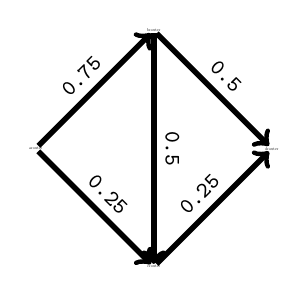
\begin{tikzpicture}
\node[scale=0.15] (a) at (0, 0) {\router{a}{router}};
\node[scale=0.15] (b) at (1.5, 1.5) {\router{b}{router}};
\node[scale=0.15] (c) at (1.5, -1.5) {\router{c}{router}};
\node[scale=0.15] (d) at (3, 0) {\router{d}{router}};
\draw[line width=2] (a) edge[above, sloped, ->] node[black,font=\bfseries] {\footnotesize \texttt{0.75}} (b);
%\draw[line width=2] (b) edge[below, sloped, bend left = 10, ->] node[black,font=\bfseries] {\tiny \texttt{0}} (a);

\draw[line width=2] (a) edge[above, sloped, ->] node[black,font=\bfseries] {\footnotesize \texttt{0.25}} (c);
%\draw[line width=2] (c) edge[below, sloped, bend left = 10, ->] node[black,font=\bfseries] {\tiny \texttt{0}} (a);

\draw[line width=2] (b) edge[above, sloped, ->] node[black,font=\bfseries] {\footnotesize \texttt{0.5}} (d);
%\draw[line width=2] (d) edge[below, sloped, bend left = 10, ->] node[black,font=\bfseries] {\tiny \texttt{0}} (b);

\draw[line width=2] (c) edge[above, sloped, ->] node[black,font=\bfseries] {\footnotesize \texttt{0.25}} (d);
%\draw[line width=2] (d) edge[below, sloped, bend left = 10, ->] node[black,font=\bfseries] {\tiny \texttt{0}} (c);

\draw[line width=2] (b) edge[above, sloped, ->] node[black,font=\bfseries] {\footnotesize \texttt{0.5}} (c);
%\draw[line width=2] (c) edge[below, sloped, bend left = 10, ->] node[black,font=\bfseries] {\tiny \texttt{0}} (b);
\end{tikzpicture}

&

\begin{tikzpicture}
\node[scale=0.15] (a) at (0, 0) {\router{a}{router}};
\node[scale=0.15] (b) at (1.5, 1.5) {\router{b}{router}};
\node[scale=0.15] (c) at (1.5, -1.5) {\router{c}{router}};
\node[scale=0.15] (d) at (3, 0) {\router{d}{router}};
\draw[line width=2] (a) edge[above, sloped, ->] node[black,font=\bfseries] {\footnotesize \texttt{0.75}} (b);
%\draw[line width=2] (b) edge[below, sloped, bend left = 10, ->] node[black,font=\bfseries] {\tiny \texttt{0}} (a);

\draw[line width=2] (a) edge[above, sloped, ->] node[black,font=\bfseries] {\footnotesize \texttt{0.25}} (c);
%\draw[line width=2] (c) edge[below, sloped, bend left = 10, ->] node[black,font=\bfseries] {\tiny \texttt{0}} (a);

\draw[line width=2] (b) edge[above, sloped, ->] node[black,font=\bfseries] {\footnotesize \texttt{0.5}} (d);
%\draw[line width=2] (d) edge[below, sloped, bend left = 10, ->] node[black,font=\bfseries] {\tiny \texttt{0}} (b);

\draw[line width=2] (c) edge[above, sloped, ->] node[black,font=\bfseries] {\footnotesize \texttt{0.25}} (d);
%\draw[line width=2] (d) edge[below, sloped, bend left = 10, ->] node[black,font=\bfseries] {\tiny \texttt{0}} (c);

\draw[line width=2] (b) edge[above, sloped, ->] node[black,font=\bfseries] {\footnotesize \texttt{0.5}} (c);
%\draw[line width=2] (c) edge[below, sloped, bend left = 10, ->] node[black,font=\bfseries] {\tiny \texttt{0}} (b);


\draw[cyan, line width=2, ->] plot [smooth] coordinates { ($(a)+(0,0.5)$) ($(b)+(0,0.75)$) ($(d)+(0,0.5)$) };

\end{tikzpicture}

&

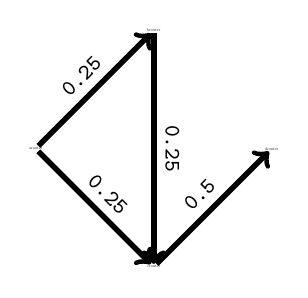
\begin{tikzpicture}
\node[scale=0.15] (a) at (0, 0) {\router{a}{router}};
\node[scale=0.15] (b) at (1.5, 1.5) {\router{b}{router}};
\node[scale=0.15] (c) at (1.5, -1.5) {\router{c}{router}};
\node[scale=0.15] (d) at (3, 0) {\router{d}{router}};
\draw[line width=2] (a) edge[above, sloped, ->] node[black,font=\bfseries] {\footnotesize \texttt{0.25}} (b);
%\draw[line width=2] (b) edge[below, sloped, bend left = 10, ->] node[black,font=\bfseries] {\tiny \texttt{0}} (a);

\draw[line width=2] (a) edge[above, sloped, ->] node[black,font=\bfseries] {\footnotesize \texttt{0.25}} (c);
%\draw[line width=2] (c) edge[below, sloped, bend left = 10, ->] node[black,font=\bfseries] {\tiny \texttt{0}} (a);

%\draw[line width=2] (b) edge[above, sloped, ->] node[black,font=\bfseries] {\footnotesize \texttt{1}} (d);
%\draw[line width=2] (d) edge[below, sloped, bend left = 10, ->] node[black,font=\bfseries] {\tiny \texttt{0}} (b);

\draw[line width=2] (c) edge[above, sloped, ->] node[black,font=\bfseries] {\footnotesize \texttt{0.5}} (d);
%\draw[line width=2] (d) edge[below, sloped, bend left = 10, ->] node[black,font=\bfseries] {\tiny \texttt{0}} (c);

\draw[line width=2] (b) edge[above, sloped, ->] node[black,font=\bfseries] {\footnotesize \texttt{0.25}} (c);
%\draw[line width=2] (c) edge[below, sloped, bend left = 10, ->] node[black,font=\bfseries] {\tiny \texttt{0}} (b);

\end{tikzpicture}

\\

(1) Solution graph

&

(2) First BFS

&

(3) Graph after reweight

\\[0.5cm]

\begin{tikzpicture}
\node[scale=0.15] (a) at (0, 0) {\router{a}{router}};
\node[scale=0.15] (b) at (1.5, 1.5) {\router{b}{router}};
\node[scale=0.15] (c) at (1.5, -1.5) {\router{c}{router}};
\node[scale=0.15] (d) at (3, 0) {\router{d}{router}};
\draw[line width=2] (a) edge[above, sloped, ->] node[black,font=\bfseries] {\footnotesize \texttt{0.25}} (b);
%\draw[line width=2] (b) edge[below, sloped, bend left = 10, ->] node[black,font=\bfseries] {\tiny \texttt{0}} (a);

\draw[line width=2] (a) edge[above, sloped, ->] node[black,font=\bfseries] {\footnotesize \texttt{0.25}} (c);
%\draw[line width=2] (c) edge[below, sloped, bend left = 10, ->] node[black,font=\bfseries] {\tiny \texttt{0}} (a);

%\draw[line width=2] (b) edge[above, sloped, ->] node[black,font=\bfseries] {\footnotesize \texttt{1}} (d);
%\draw[line width=2] (d) edge[below, sloped, bend left = 10, ->] node[black,font=\bfseries] {\tiny \texttt{0}} (b);

\draw[line width=2] (c) edge[above, sloped, ->] node[black,font=\bfseries] {\footnotesize \texttt{0.5}} (d);
%\draw[line width=2] (d) edge[below, sloped, bend left = 10, ->] node[black,font=\bfseries] {\tiny \texttt{0}} (c);

\draw[line width=2] (b) edge[above, sloped, ->] node[black,font=\bfseries] {\footnotesize \texttt{0.25}} (c);
%\draw[line width=2] (c) edge[below, sloped, bend left = 10, ->] node[black,font=\bfseries] {\tiny \texttt{0}} (b);

\draw[cyan, line width=2, ->] plot [smooth] coordinates { ($(a)+(0,-0.5)$) ($(c)+(0,-0.75)$) ($(d)+(0,-0.5)$) };


\end{tikzpicture}

&

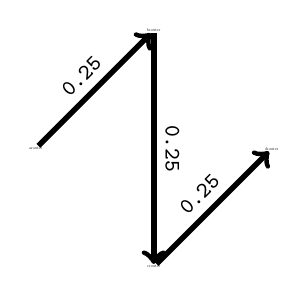
\begin{tikzpicture}
\node[scale=0.15] (a) at (0, 0) {\router{a}{router}};
\node[scale=0.15] (b) at (1.5, 1.5) {\router{b}{router}};
\node[scale=0.15] (c) at (1.5, -1.5) {\router{c}{router}};
\node[scale=0.15] (d) at (3, 0) {\router{d}{router}};
\draw[line width=2] (a) edge[above, sloped, ->] node[black,font=\bfseries] {\footnotesize \texttt{0.25}} (b);
%\draw[line width=2] (b) edge[below, sloped, bend left = 10, ->] node[black,font=\bfseries] {\tiny \texttt{0}} (a);

%\draw[line width=2] (a) edge[above, sloped, ->] node[black,font=\bfseries] {\footnotesize \texttt{1}} (c);
%\draw[line width=2] (c) edge[below, sloped, bend left = 10, ->] node[black,font=\bfseries] {\tiny \texttt{0}} (a);

%\draw[line width=2] (b) edge[above, sloped, ->] node[black,font=\bfseries] {\footnotesize \texttt{1}} (d);
%\draw[line width=2] (d) edge[below, sloped, bend left = 10, ->] node[black,font=\bfseries] {\tiny \texttt{0}} (b);

\draw[line width=2] (c) edge[above, sloped, ->] node[black,font=\bfseries] {\footnotesize \texttt{0.25}} (d);
%\draw[line width=2] (d) edge[below, sloped, bend left = 10, ->] node[black,font=\bfseries] {\tiny \texttt{0}} (c);

\draw[line width=2] (b) edge[above, sloped, ->] node[black,font=\bfseries] {\footnotesize \texttt{0.25}} (c);
%\draw[line width=2] (c) edge[below, sloped, bend left = 10, ->] node[black,font=\bfseries] {\tiny \texttt{0}} (b);

%\draw[cyan, line width=2, ->] plot [smooth] coordinates { ($(a)+(0,-0.5)$) ($(c)+(0,-0.75)$) ($(d)+(0,-0.5)$) };


\end{tikzpicture}

&

\begin{tikzpicture}
\node[scale=0.15] (a) at (0, 0) {\router{a}{router}};
\node[scale=0.15] (b) at (1.5, 1.5) {\router{b}{router}};
\node[scale=0.15] (c) at (1.5, -1.5) {\router{c}{router}};
\node[scale=0.15] (d) at (3, 0) {\router{d}{router}};
\draw[line width=2] (a) edge[above, sloped, ->] node[black,font=\bfseries] {\footnotesize \texttt{0.25}} (b);
%\draw[line width=2] (b) edge[below, sloped, bend left = 10, ->] node[black,font=\bfseries] {\tiny \texttt{0}} (a);

%\draw[line width=2] (a) edge[above, sloped, ->] node[black,font=\bfseries] {\footnotesize \texttt{1}} (c);
%\draw[line width=2] (c) edge[below, sloped, bend left = 10, ->] node[black,font=\bfseries] {\tiny \texttt{0}} (a);

%\draw[line width=2] (b) edge[above, sloped, ->] node[black,font=\bfseries] {\footnotesize \texttt{1}} (d);
%\draw[line width=2] (d) edge[below, sloped, bend left = 10, ->] node[black,font=\bfseries] {\tiny \texttt{0}} (b);

\draw[line width=2] (c) edge[above, sloped, ->] node[black,font=\bfseries] {\footnotesize \texttt{0.25}} (d);
%\draw[line width=2] (d) edge[below, sloped, bend left = 10, ->] node[black,font=\bfseries] {\tiny \texttt{0}} (c);

\draw[line width=2] (b) edge[above, sloped, ->] node[black,font=\bfseries] {\footnotesize \texttt{0.25}} (c);
%\draw[line width=2] (c) edge[below, sloped, bend left = 10, ->] node[black,font=\bfseries] {\tiny \texttt{0}} (b);

\draw[cyan, line width=2, ->] plot [smooth] coordinates { ($(a)+(0,0.5)$) ($(b)+(0,0.75)$) ($(b)+(0.75,0)$)  ($(b)+(0,-1)$) ($(c)+(-0.75,0)$) ($(c)+(0,-0.75)$) ($(d)+(0,-0.75)$)};

\end{tikzpicture}


\\

(4) Second BFS

&

(5) Graph after reweight

&

(6) Third BFS

\end{tabular}
\end{center}
\caption{Converting the flow to a path set.}
\label{fig:flow-path}
\end{figure}

Using this procedure, we can easily transform a solution of \mcflp~in a solution 
$\mathcal{P}_1, \ldots, \mathcal{P}_r$ of Problem \ref{prob:tep-mul}. Algorithm \ref{algo:mcf-seg} provides a formal description
of this process.

%To implement such a solution 
%on a network with segment routing we can simply use our minimum segmentation algorithm.
% on how we can combine \mcflp~with
%the minimum segmentation algorithm to provide an optimal solution to Problem \ref{prob:tep-mul}
%implementable with segment routing.

\begin{algorithm}[t]
\small
\caption{$\textsf{TE-multipath}\left( G, \mathcal{D} \right)$}
\begin{algorithmic}[1]
\STATE $x, y, \lambda \gets \textsf{LP-SOLVE}(\textsf{MCF-LP}(G, \mathcal{D}))$ \label{line:srmcf_lp}
\STATE $\mathcal{P} \gets \emptyset$
\FOR{$d \in \mathcal{D}$}
  \STATE $G_d \gets (V, \{ e \in E(G) \mid x_{ed} > 0 \})$ \label{line:srmcf_buildg}
  \STATE $p \gets \textsf{BFS}(G_d, src(d), dst(d))$ \label{line:srmcf_p1}
  \WHILE{$p \neq \bot$} \label{line:srmcf_while}
    \STATE $\Delta \gets \min_{e \in E(p)} x_{ed}$ \label{line:srmcf_delta}
    \STATE $\mathcal{P} \gets \mathcal{P} \cup \{ (p, \Delta) \}$ \label{line:srmcf_add}
    \FOR{$e \in E(p)$} \label{line:srmcf_for}
      \STATE $x_{ed} \gets x_{ed} - \Delta$ \label{line:srmcf_update}
    \ENDFOR
    \STATE $G_d \gets (V, \{ e \in E(G) \mid x_{ed} > 0 \})$ \label{line:srmcf_buildgw}
    \STATE $p \gets \textsf{BFS}(G_d, src(d), dst(d))$ \label{line:srmcf_pw}
  \ENDWHILE
\ENDFOR
\RETURN $\lambda$, $\mathcal{P}$
\end{algorithmic}
\label{algo:mcf-seg}
\end{algorithm}

\begin{proposition}
Algorithm \ref{algo:mcf-seg} runs in polynomial time and computes an optimal solution of Problem \ref{prob:tep-mul}.
\end{proposition}

\begin{proof}
Optimality comes from the fact that $\mcflp$ correctly models Problem \ref{prob:tep-mul} \cite{MCF}.

We know that linear problems can be solved in polynomial time \cite{lp1, lp2}. Therefore $x$ can be computed in polynomial time on line \ref{line:srmcf_lp}.
It remains to show that our path building process takes polynomial time. Let $d \in \mathcal{D}$. Building the graph $G_d$ on line \ref{line:srmcf_buildg} takes
$O(|E(G)| \cdot |\mathcal{D}|)$ and each \textsf{BFS} call takes $O(|G|)$. In  the body of the while loop, that is, lines \ref{line:srmcf_delta}
to \ref{line:srmcf_pw}, the most costly line is line \ref{line:srmcf_pw} which takes $O(|V(G)| \cdot |E(G)|)$. Therefore we only need to prove that the number 
of iterations of the while loop is polynomial. Since $\Delta = \min_{e \in E(p)} x_{ed}$, at each iteration, at least one edge is removed from $G_d$ at
line \ref{line:srmcf_buildgw}. This means that the number of iterations of the while loop is at most $|E(G)|$.
%giving a total runtime of $O(LP + |\mathcal{D}| \cdot (|G| + |E(G)| \cdot |G|)) = O(LP + |\mathcal{D}| \cdot |G| \cdot |E(G)|)$.
\end{proof}

By requiring integral variables on model $\mcflp(G, \mathcal{D})$, that is, by replacing $x_{ed} \in [0, 1]$  by $x_{ed} \in \{ 0, 1 \}$, we obtain 
a model for solving Problem \ref{prob:tep}. This illustrates that just by requiring integer variables we can completely change the difficulty of the problem
since it takes us from a polynomial solvable problem to a \NPhard~one in this case.

%As with any solution that consists of solving a problem on the original network $G$ and only after segments the paths,
%this solutions has the huge drawback that it fails to provide control on the number of segments needed to implement the 
%solution. We executed this algorithm on our data set and analysed the number of segments necessary in these solutions.

%\todo{show plots and discuss}


\section{Traffic engineering with segment routing}

In this section we discuss the variants of Problems \ref{prob:tep} and \ref{prob:tep-mul} when
instead of using arbitrary paths for routing, we use sr-paths. The SR version of the TE problem is
obtained by replacing paths by sr-paths, $\cnt(p_i, e)$ by $\r(\sr{p}_i, e)$ and adding a constraint on the segment cost of 
the sr-paths found. Recall that $\r(\sr{p}_i, e)$ was defined on Chapter \ref{chapter:sr-optimal} and represents the 
proportion of the traffic that traverses edge $e$ when routing over sr-path $\sr{p}$.

This last constraint is important to ensure that the paths can be supported by the routers in the network.
This leads to the definition of the following two problems which, respectively, correspond to Problems \ref{prob:tep} and \ref{prob:tep-mul}.

\begin{problem}{Segment routing traffic engineering}
\label{prob:srte}
\textbf{Input:} A network $G$, a set of demands $\mathcal{D} = \{d_1, \ldots, d_n\}$ on $G$ and $k \in \mathbb{N}$.

\textbf{Output:} The minimum factor $\lambda \geq 0$ and set of sr-paths on $G$, $\sr{p}_1, \ldots, \sr{p}_n$ such that $\sr{p}_i$ is a 
sr-path from $s_i$ to $t_i$ with $\cost(\sr{p}_i) \leq k $ and for each link $e \in E(G)$ it holds
$$
\sum_{i = 1}^n \r(\sr{p}_i, e) \cdot \vol(d_i) \leq \lambda \cdot \bnd(e).
$$ 
\end{problem}

\begin{problem}{Segment routing traffic engineering}
\label{prob:srte-mul}
\textbf{Input:} A network $G$, a set of demands $\mathcal{D} = \{d_1, \ldots, d_n\}$ on $G$ and $k \in  \mathbb{N}$.

\textbf{Output:} The minimum factor $\lambda \geq 0$ and set of sr-paths on $G$, $\sr{\mathcal{P}}_1, \ldots, \sr{\mathcal{P}}_n$ such that
$\sr{\mathcal{P}}_i$ is a 
non-empty set of pairs $(\sr{p}, f)$ where $\sr{p}$ sr-path from $s_i$ to $t_i$ with $\cost(\sr{p}_i) \leq k $, $f \in [0, 1]$ and for each link $e \in E(G)$ it holds
$$
\sum_{i = 1}^n \sum_{(\sr{p}, f) \in \sr{\mathcal{P}}_i} f \cdot \r(\sr{p}, e) \cdot \vol(d_i) \leq \lambda \cdot \bnd(e).
$$ 
\end{problem}

The minimum segmentation algorithm provides a way to translate solutions of Problems \ref{prob:tep} and \ref{prob:tep-mul}
into solutions of Problems \ref{prob:srte} and \ref{prob:srte-mul}, respectively. The advantage of this approach is that
makes it possible to leverage existing algorithms for solving these widely studied graph problems. The drawback of course
is that since these algorithms are oblivious to segment routing, there is no way of knowing whether or not the output paths will
require too many segments for routers to be able to support them.

We first evaluate the segment cost mentioned above. 
We already did this in the previous chapter when we considered the problem of computing minimum latency sr-paths.
This is a way to evaluate how necessary it is to develop dedicated algorithms and how often we can get away by
simply segmenting graph centric solutions using the minimum segmentation algorithm proposed in Chapter \ref{chapter:sr}.
Perhaps in the future routers will be able to support a high amount of segments
and whenever this is the case, it will become fruitless to develop dedicated algorithms.

% We used the dataset from the Repetita project to evaluate the segment cost of solutions to Problem \ref{prob:tep}. For each topology
% we executed Algorithm \ref{algo:mcf-seg} defined in the previous section and segment all the paths from the solution. Figure 
% \ref{fig:minseg_MCF} shows a CDF  of the maximum segment cost of minimum segmentation the path sets correspond to each demands,
% over all topologies.
% 
% \begin{figure}
% \begin{center}
% 
\includegraphics[scale=0.6]{./Network-lib/data/plot/todo.pdf}
% \end{center}
% \caption{CDF of the segment cost of the minimal segmentations of solution computed with Algorithm \ref{algo:mcf-seg}.}
% \label{fig:minseg_MCF}
% \end{figure}


\subsection{Existing MIP models and algorithms for SRTE}

We now have all the tools needed to describe existing models for the traffic engineering problem with segment routing.
The first approach that was developed by Bathia et al and considers only sr-paths of the form $\langle s, x, t \rangle$ to route a demand from
$s$ to $t$ \cite{bhatia}. That is, it restricts the set of admissible sr-paths to sr-paths with a single detours towards a given
router $x$ on the network. The main advantage of doing this is that we obtain a very efficient model since for each demand 
there is a single decision to make: which intermediate router to use.

% To simplify the notations and model formulations, it is convenient to define the set of all sr-paths with a segment cost lower
% than a given constant.
% 

% 
% With this notation,

Let $\PB = \left\{ \langle \src(d), x, \dst(d) \rangle \mid x \in V(G) \right\}$. We define binary variables $x_{dp}$ such that $x_{dp} = 1$ if and only if demand $d$ is routed
over sr-path $p$.  Their model can be formulated as follows.

\begin{center}
\begin{tabular}{crcllr}
\multicolumn{5}{l}{$\bhatia(G, \mathcal{D})$} \\[0.5cm] 
$\displaystyle \mathbf{min}$ & $\lambda$ & & & & \\[0.5cm]
$\textbf{s.t.}$ & $\displaystyle \sum_{p \in \PB} x_{d p}$ & $=$ & $1$ & $\forall d \in \mathcal{D}$ \\[0.5cm] 
& $\displaystyle \sum_{\sr{p} \in \PB} \sum_{d \in \mathcal{D}} \r(\sr{p}, e)  \cdot \vol(d) \cdot x_{dp}$ & $\leq$ & $\lambda \cdot \bnd(e)$ & $\forall e \in E(G)$ \\[0.5cm]
& $x_{dp} \in \{ 0, 1 \}$ & & & $\forall p \in \PB, \ \forall d \in \mathcal{D}$
\end{tabular}
\end{center}


The first set of constraints specifies that each demand has to be served by exactly one path. The second set of constraints ensures that no edge 
carries more than $\lambda \cdot \bnd(e)$ traffic.

The model that we use for our column generation solution is a generalization of this one where we replace the set of paths considered, $\PB$
by the set of all sr-paths with at most a given segment cost, $\mathcal{\sr{P}}_k(G)$. 
Renaud Hartert already had proposed this generalization in his thesis \cite{hartert18}. The only difference between his model and ours is that we also
consider adjacency segments in our sr-paths whereas his model only considered node segments. We discuss our model in more detail in the next section.

In his thesis, Hartert also proposed another model called \emph{segment model}. This model is closely related to the IP version of the model that we presented for the
multi-commodity flow \mcflp. In the integral MCF model, we use variables $x_{ed}$ to indicate whether demand $d$ is routed though edge $e$. Then
we use classic flow conservation constraints to ensure that if $x_{ed} = 1$ then we have a path $(e_1, \ldots, e_l)$ starting at
$\src(d)$ and ending at $\src(d)$ such that $x_{e_1 d} = 1, \ldots, x_{e_l d} = 1$. In the segment model, instead of edges we consider the shortest
path subgraphs. Concretely, we use variables $x^d_{u v}$ for $d \in \mathcal{D}, u, v \in V(G)$
defined such that $x^d_{u v} = 1$ if and only demand $d$ is routed over the shortest paths between nodes $u$ and $v$, that is, the subgraph $\sp(u, v)$. 
Then we use the same flow conservation constraints to ensure that whenever $x^d_{uv} = 1$ then there exists a sequence of nodes
$(v_1 = s, v_2, \ldots, v_k = t)$ such that $x^d_{v_1 v_2} = x^d_{v_2 v_3} = \ldots = x^d_{v_{k - 1} v_k} = 1$ meaning that we route the demand
$d$ by following the shortest paths from $v_1$ to $v_2$, then from $v_2$ to $v_3$ and so on. In other words, we use sr-path 
$\langle v_1, v_2, \ldots, v_k \rangle$ to route $d$.

\begin{center}
\begin{tabular}{rcllr}
\multicolumn{5}{l}{$\srteseg(G, \mathcal{D})$} \\[0.5cm] 
\multicolumn{3}{l}{$\mathbf{min} \quad \lambda$} & $\textbf{s.t.}$ & \\[0.5cm]
$\displaystyle \sum_{d = 1}^r \sum_{u, v \in V(G) : u \neq v} x^d_{uv} \cdot \r(u, v, e) \cdot \vol(d)$ & $\leq$ & $\lambda \cdot \bnd(e)$ & $\forall e \in E(G)$ & \\[0.5cm]
$\displaystyle \sum_{u \in V(G) \setminus \{ v \}} x^d_{uv} - \sum_{u \in V(G) \setminus \{ v \}} x^d_{vu}$ & $=$    &  $0$ & $\forall d = (s, t, \nu) \in \mathcal{D}$, & \\[-0.2cm]
& & & $\forall v \in V(G) \setminus \{ s, t \}$ & \\[0.5cm]
$\displaystyle \sum_{u \in V(G) \setminus \{ s \}} x^d_{us} - \sum_{u \in V(G) \setminus \{ s \}} x^d_{us}$ & $=$    & $-1$ & $\forall i \in \{ 1, \ldots, r \}$, \\[-0.2cm]
& & & $\forall d = (s, t, \nu) \in \mathcal{D}$ \\[0.5cm]
$\displaystyle \sum_{u \in V(G) \setminus \{ t \}} x^d_{ut} - \sum_{u \in V(G) \setminus \{ t \}} x^d_{ut}$ & $=$    &  $1$ & $\forall i \in \{ 1, \ldots, r \}$, \\[-0.2cm]
& & & $\forall d = (s, t, \nu) \in \mathcal{D}$ \\[0.5cm] 
$x^d_{uv}$  &    $\in$    &  $\{0, 1\}$  & $\forall e \in E(G), \ \forall d \in \mathcal{D}$ & \\[0.5cm]
$\lambda \geq 0$ & & & &    
\end{tabular}
\end{center}


As it is, this model does not make any guarantees on the number of segments used to route a demand. We can overcome this by adding the following additional constraint
limiting the maximum number of node segments in the sr-paths to $k$:

$$
\sum_{u, v \in V(G) : u \neq v} x^d_{u, v} \leq k \quad \forall d \in \mathcal{D}.
$$

In all these models, by relaxing the integrability constraints to allow the variables to take any real value in $[0, 1]$ we automatically get a polynomial time solvable
LP for Problem \ref{prob:srte-mul} (over the restricted set of sr-paths that each model considers). 

\subsubsection*{Model comparison}

Due to its simplicity, optimal solutions of $\bhatia$ can be computed very efficiently. It it a relaxation of Problem \ref{prob:srte} because it significantly restricts the
sets of sr-paths that can be used by considering only paths in $P_1$. The generalization of this model consisting of replacing $P_1$ by $\mathcal{\sr{P}}_k$ removes this 
restriction by considering any possible sr-path whose segment cost is at most $k$ to route any given demand. The problem of this model is that it contains a number of variables
which is exponential with respect to $k$ since $|\Pk| = O(|G|^k)$. This means that even for small values of $k$ it will not scale. Hartert showed in his thesis that even for $k \geq 3$ the number of 
variables is too big to allow good solutions to be found in a reasonable amount of computation time. We will show how we use column generation to overcome this problem the next section.

The segment model presented above overcomes this problem by implicitly representing sr-paths with flow conservation constraints. With this, it manages
to model sr-paths of segment cost up to $k$ using only $|V(G)|^2 \cdot |\mathcal{D}|$ variables. One drawback of this solution is that it
cannot represent sr-paths containing adjacency segments. Moreover, it turns out that on the larger topologies this model quickly becomes too large as well. This is not
surprising since with one demand per pair of nodes the total number of variables is about $|V(G)|^4$.

Other researchers have proposed heuristic techniques for solving Problem \ref{prob:srte}. Hartert et al. proposed in DEFO \cite{defo,hartert2015solving} a Large
Neighborhood Search technique combined with Constraint Programming. Later, Gay et al. proposed in \cite{steven} to use standard local search to iteratively improve the current solution. 
These heuristic approaches are rather efficient but provide no way of knowing how far from the optimal value they end up.
Moreover, all the existing approaches only consider node segments in their formulation. They are thus not able to fully exploit the flexibility of segment routing with adjacency segments.
Not only that but we have shown in our experiments that, on instances where only a few routing configuration lead to good solution, these heuristic approaches have difficulty of finding them. 
This is a common drawback of LS since in such cases it becomes very unlikely for the search to be able to reach these very precise configurations.


\section{The idea behind Column Generation}

% \todo{
% Structure: 1. Explain LP duality. 2. show that removing variables from primal = remove constraints from dual. 3. constraints is easier to check, with a partial solution
% of the primal we can map to the dual and check for constraints viaolation. if not violation optimal. maybe show concrete example before.
% }
% 
% 
% Strong duality \todo{ref} tell us that there exists another LP, called the dual, and that for any feasible solution $x$
% of the primal

We now describe how we used Column Generation (CG) \cite{desaulniers2006column} to overcome the model size problems faced when using the path model for
solving the traffic engineering problem with SR. CG is usually used to solve linear programs with a huge number of variables. The idea is to solve the problem for a subset
of the variables and then incrementally insert the missing variables, slowly growing the model. Each time that we add new variables, we solve the model again to check
for optimality. One could ask what
is the point of doing this since at some point we will have the whole set of variables, so why not just solve the full problem instead? However, we will carefully select the 
new variables that we introduce so that in general this framework will reach an optimal solution to the original \emph{problem without ever needing to consider all variables}.

To understand the impact of ignoring a variable and how we can prove optimality without considering all variables, we work out a small example. 
This will allow us to explain the main idea behind CG in a much more 
intuitive way by providing an example without overwhelming mathematical notations. Suppose that we have the following LP that we want to solve.

\begin{center}
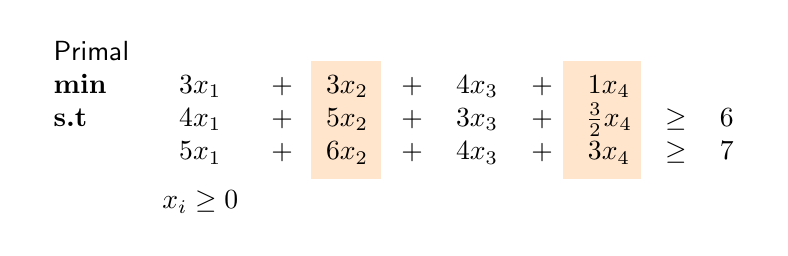
\begin{tikzpicture}
\def\x{0}
\def\y{0}
\fill[orange!20!white] (\x + 4 - 0.4, \y + 0 - 0.425) rectangle (\x + 4.9 - 0.4, \y + -1.5 - 0.425);
\fill[orange!20!white] (\x + 7.2 - 0.4, \y + 0 - 0.425) rectangle (\x + 8.1 - 0.3, \y + -1.5 - 0.425);
\node[anchor=north west] (primal) at (\x, \y) {
\begin{tabular}{lcccccccccc}
\textsf{Primal} & & & & & & & & & \\
$\displaystyle \mathbf{min}$ & $3 x_1$ & $+$ & $3 x_2$ & $+$ & $4 x_3$ & $+$ & $1 x_4$ & & \\
\textbf{s.t} & $4 x_1$ & $+$ & $5 x_2$ & $+$ & $3 x_3$ & $+$ & $\frac{3}{2} x_4$ & $\geq$ & $6$ \\
             & $5 x_1$ & $+$ & $6 x_2$ & $+$ & $4 x_3$ & $+$ & $3 x_4$ & $\geq$ & $7$ \\[0.2cm]
& $x_i \geq 0$ & & & & & & & &
\end{tabular}
};
\end{tikzpicture}
\end{center}

The dual of this problem can be obtained by following a systematic procedure. By doing so, we obtain the following linear program.
\begin{center}
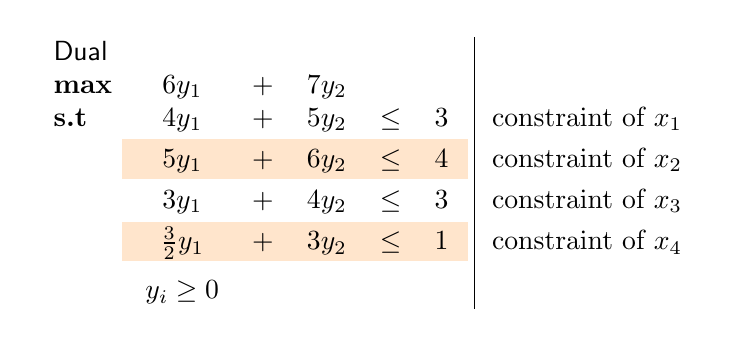
\begin{tikzpicture}
\def\x{0}
\def\y{0}
\fill[orange!20!white] (\x + 2 - 0.8, \y + -1 - 0.425) rectangle (\x + 5.6, \y + -1.5 - 0.425);
\fill[orange!20!white] (\x + 2 - 0.8, \y + -1.2 - 3 * 0.425) rectangle (\x + 5.6, \y + -1.7 - 3 * 0.425);
\node[anchor=north west] (dual) at (\x, \y) {
\begin{tabular}{lccccc | r}
\textsf{Dual} & & & & & \\
$\mathbf{max}$ & $6 y_1$ & $+$ & $7 y_2$ & &  \\
\textbf{s.t} & $4 y_1$ & $+$ & $5 y_2$ & $\leq$ & $3$ \quad & constraint of $x_1$ \\[0.1cm]
             & $5 y_1$ & $+$ & $6 y_2$ & $\leq$ & $4$ \quad  & constraint of $x_2$ \\[0.1cm]
             & $3 y_1$ & $+$ & $4 y_2$ & $\leq$ & $3$ \quad  & constraint of $x_3$ \\[0.1cm]
             & $\frac{3}{2} y_1$ & $+$ & $3 y_2$ & $\leq$ & $1$  \quad  & constraint of $x_4$ \\[0.2cm]
& $y_i \geq 0$ & & & &
\end{tabular}
};
\end{tikzpicture}
\end{center}

Each variable $x_i$ of the primal corresponds to a constraints of the dual. So, for instance, $x_2$ corresponds to constraint
$5 y_1 + 6 y_2 \geq 4$ and $x_4$ corresponds to the constraint $\frac{3}{2} y_1 + 3 y_2 \geq 1$ as highlighted in the models.

Because of this correspondence, when we ignore a variable on the primal, this translates in the dual to ignoring the corresponding constraint. 
For example, if we consider the restricted primal problem on variables $x_1$ and $x_3$ only (that we denote by $\textsf{Primal}(1, 3)$), 
and we take the dual, the dual will be the same as above but 
will only have the first and third constraints.

\begin{center}
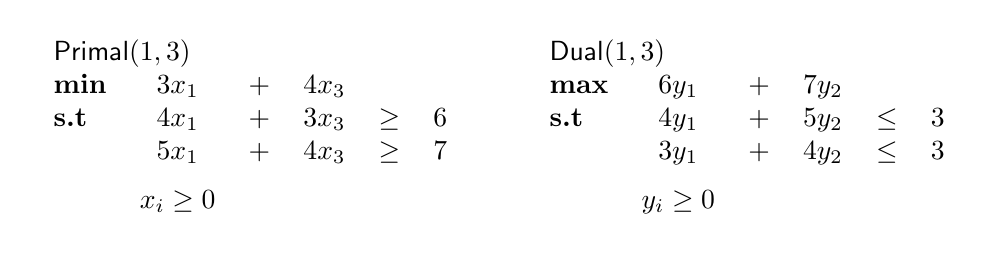
\begin{tikzpicture}
\def\x{0}
\def\y{0}
\node[anchor=north west] (primal) at (\x, \y) {
\begin{tabular}{lcccccccccc}
\multicolumn{11}{l}{$\textsf{Primal}(1, 3)$} \\
$\mathbf{min}$ & $3 x_1$  & $+$ & $4 x_3$ & & \\
\textbf{s.t} & $4 x_1$  & $+$ & $3 x_3$ & $\geq$ & $6$ \\
& $5 x_1$ & $+$ & $4 x_3$ & $\geq$ & $7$ \\[0.2cm]
& $x_i \geq 0$ & & & &
\end{tabular}
};

\def\x{6.3}
\def\y{0}
\node[anchor=north west] (dual) at (\x, \y) {
\begin{tabular}{lccccc}
\multicolumn{6}{l}{$\textsf{Dual}(1, 3)$} \\
$\mathbf{max}$ & $6 y_1$ & $+$ & $7 y_2$ & &  \\
\textbf{s.t} & $4 y_1$ & $+$ & $5 y_2$ & $\leq$ & $3$ \\
& $3 y_1$ & $+$ & $4 y_2$ & $\leq$ & $3$ \\[0.2cm]
& $y_i \geq 0$ & & & &
\end{tabular}
};
\end{tikzpicture}
\end{center}

Suppose that we solve the restricted primal we obtain the optimal solution $x^* = (1.5, 0)$. By duality, we also obtain 
an optimal solution $y^*$ of the restricted dual. In this case $y^* = (0.75, 0)$. From here, we want to be able to decide whether $x^*$ is actually optimal
for the original primal problem and, if not, what new variable $x_2$ or $x_4$ should we consider to improve the solution. By strong
duality, we know that $x^*$ is optimal for \textsf{Primal} if and only if $y^*$ is optimal for \textsf{Dual}. Since the only 
difference between \textsf{Dual} and $\textsf{Dual}(1, 3)$ is that we removed two constraints from \textsf{Dual}, $y^*$
contains values for \emph{all} variables of the dual. Therefore,
to check the optimality of $y^*$ for \textsf{Dual}, we can plug its values into the missing constraints to check whether $y^*$ satisfies them. 
If $y^*$ happens to satisfy all of them, then it must be optimal for the unrestricted dual and by consequence, $x^*$ is optimal for the
unrestricted original primal.
In this example, for the constraint corresponding to $x_2$ we have
\begin{align*}
5 y_1 + 6 y_2 = 5 \cdot 0.75 + 6 \cdot 0 = 3.75 > 3
\end{align*}
and for the constraint corresponding to $x_4$ we have
\begin{align*}
2 y_1 + 6 y_2 = 2 \cdot 0.75 + 6 \cdot 0 = 1.5 > 1. \\
\end{align*}
Both of them are violated so we cannot conclude that $y^*$ is optimal for \textsf{Dual}. So we chose one of $x_2, x_4$ to be added to the model.
For the sake of example, we choose $x_2$ obtaining (we highlighted in green the newly added column):

\begin{center}
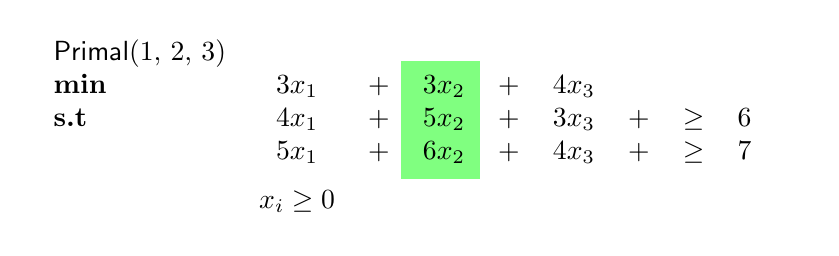
\begin{tikzpicture}
\def\x{0}
\def\y{0}
\fill[green!50!white] (\x + 4 + 1.15 - 0.4, \y + 0 - 0.425) rectangle (\x + 5 + 1.15 - 0.4, \y + -1.5 - 0.425);
\node[anchor=north west] (dual) at (\x, \y) {
\begin{tabular}{lcccccccccc}
\textsf{Primal}(1, 2, 3) & & & & & & &  \\
$\displaystyle \mathbf{min}$ & $3 x_1$ & $+$ & $3 x_2$ & $+$ & $4 x_3$ & & \\
\textbf{s.t} & $4 x_1$ & $+$ & $5 x_2$ & $+$ & $3 x_3$ & $+$ & $\geq$ & $6$ \\
             & $5 x_1$ & $+$ & $6 x_2$ & $+$ & $4 x_3$ & $+$ & $\geq$ & $7$ \\[0.2cm]
& $x_i \geq 0$ & & & & & & & &
\end{tabular}
};
\end{tikzpicture}
\end{center}

Solving this yields a primal solution $x^* = (0, 1.2, 0)$ and dual solution
$y^*(0.6, 0)$. As before, we check whether this solution is optimal for the 
original problem by checking whether it satisfies the remaining constraints.
In this case we only have one constraint left, the one corresponding to $x_4$.
By plugging into it the values of $y^*$ we get
\begin{align*}
\frac{3}{2} y_1 + 3 y_2 = \frac{3}{2} \cdot 0.6 + 3 \cdot 0 = 0.9 \leq 1. \\
\end{align*}
The constraint is satisfied so we conclude that $y^*$ is optimal for
\textsf{Dual} and by strong duality we conclude that $x^* = (0, 1.2, 0, 0)$
is optimal for \textsf{Primal} (note that we added a value of $0$ for 
all ignored variables).

With this process, we were able to solve \textsf{Primal} without ever having
to consider $x_4$. Of course this is just a small illustrative example so the gain is not
significant but, on larger models with a huge amount of variables, this can save huge amounts of computation
time. This finished our introductory example about column generation. 

We are now going to abstract from it and describe the general approach. Lets write the problem we are aiming to solve
in the following general form

\begin{center}
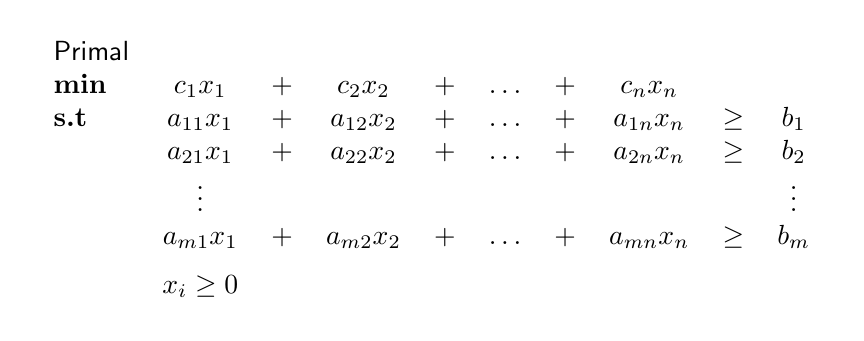
\begin{tikzpicture}
\def\x{0}
\def\y{0}
\node[anchor=north west] (primal) at (\x, \y) {
\begin{tabular}{lcccccccccc}
\textsf{Primal} & & & & & & & & & \\
$\displaystyle \mathbf{min}$ & $c_1 x_1$ & $+$ & $c_2 x_2$ & $+$ & $\ldots$ & $+$ & $c_n x_n$ & & \\
\textbf{s.t} & $a_{11} x_1$ & $+$ & $a_{12} x_2$ & $+$ & $\ldots$ & $+$ & $a_{1n} x_n$ & $\geq$ & $b_1$ \\
             & $a_{21} x_1$ & $+$ & $a_{22} x_2$ & $+$ & $\ldots$ & $+$ & $a_{2n} x_n$ & $\geq$ & $b_2$ \\
             & $\vdots$ & & & & & & & & $\vdots$ \\
             & $a_{m1} x_1$ & $+$ & $a_{m2} x_2$ & $+$ & $\ldots$ & $+$ & $a_{mn} x_n$ & $\geq$ & $b_m$ \\[0.2cm]
& $x_i \geq 0$ & & & & & & & &
\end{tabular}
};
\end{tikzpicture}
\end{center}

whose dual is easily shown to be

\begin{center}
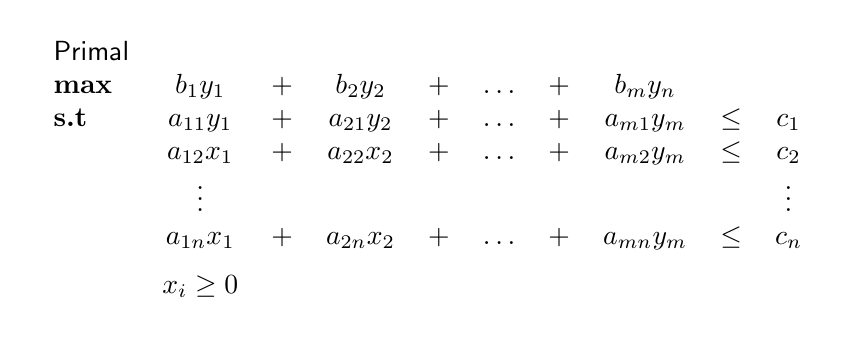
\begin{tikzpicture}
\def\x{0}
\def\y{0}
\node[anchor=north west] (primal) at (\x, \y) {
\begin{tabular}{lcccccccccc}
\textsf{Primal} & & & & & & & & & \\
$\displaystyle \mathbf{max}$ & $b_1 y_1$ & $+$ & $b_2 y_2$ & $+$ & $\ldots$ & $+$ & $b_m y_n$ & & \\
\textbf{s.t} & $a_{11} y_1$ & $+$ & $a_{21} y_2$ & $+$ & $\ldots$ & $+$ & $a_{m1} y_m$ & $\leq$ & $c_1$ \\
             & $a_{12} x_1$ & $+$ & $a_{22} x_2$ & $+$ & $\ldots$ & $+$ & $a_{m2} y_m$ & $\leq$ & $c_2$ \\
             & $\vdots$ & & & & & & & & $\vdots$ \\
             & $a_{1n} x_1$ & $+$ & $a_{2n} x_2$ & $+$ & $\ldots$ & $+$ & $a_{mn} y_m$ & $\leq$ & $c_n$ \\[0.2cm]
& $x_i \geq 0$ & & & & & & & &
\end{tabular}
};
\end{tikzpicture}
\end{center}

In general, we need a better way
for finding a new variable to introduce. In the previous example we did it by iterating over all remaining variables
and checking the corresponding constraint. Since CG is a framework that we want to use when we have a \emph{huge} amount of 
variables, this process is not realistic as it will involve checking the same amount of constraints. The idea to overcome this
is to express the problem of finding the variable as a another optimization problem which hopefully translates into something
that is solvable by an algorithm that is faster than a simple brute-force iterations on the missing variables.

The first step to achieve this is to express the condition for a new variable to be a candidate mathematically. Keeping the notation
used in the example, we see that each variable $x_i$ is associated to a column of coefficients $c_i, a_{1i}, a_{2i}, \ldots, a_{mi}$
where the first is the objective function coefficient and the others are the constraints coefficients in the primal.
The constraint associated to $x_i$ is the dual is given by
$$
a_{1i} + a_{2i} + \ldots + a_{mi} = \sum_{j = 1}^m a_{ji} y_i \leq c_i.
$$
Checking whether it is violated, or in other words, whether $x_i$ needs to be considered in the \textsf{Primal}, consists of 
checking whether
$$
\sum_{j = 1}^m a_{ji} y_i > c_i \Leftrightarrow \sum_{j = 1}^m a_{ji} y_i - c_i > 0.
$$

If we let $I$ be the set of indexes of the variables that we consider at a given point in the \textsf{Primal}, then the problem
of finding a new variable can be expressed as finding $i \in \{ 1, \ldots, n\} \setminus I$ such that
$$
\sum_{j = 1}^m a_{ji} y_i - c_i > 0.
$$
Therefore, if we compute the index $i^* \in \{ 1, \ldots, n\} \setminus I$ for which the value
$$
\sum_{j = 1}^m a_{ji^*} y_{i^*} - c_{i^*}
$$
is \emph{maximum} we know that there exists a new variable that we need to consider if and only if
$$
\sum_{j = 1}^m a_{ji^*} y_{i^*} - c_{i^*} > 0.
$$

Therefore, we can solve the problem of finding a new variable to add by solving the problem
$$
\max_{i \in \{ 1, \ldots, n\} \setminus I} \quad \sum_{j = 1}^m a_{ji} y_{i} - c_{i}.
$$
At first sight this problem might not seem any easier to solve than iterating over all $i \in \{ 1, \ldots, n\} \setminus I$
and computing the maximum but in practice this problem ofter has a nice structure and is usually solvable 
by a better, more efficient, algorithm than a simple brute force iteration. This problem is often referred to as the
\emph{pricing problem}.

Figure \ref{fig:col-gen-schema} provides a schematic vision of the column generation process.
CG generation is a very wide field and what we described here is just a very small glimpse into it \cite{desaulniers2006column}.
It is also important to note that what we did here only applies to \emph{continuous} linear programs and not to integer programming.
Therefore, we can only use this to compute solutions of LP that contain no integer variables. In order to obtain optimal
integral solution we need to add another layer to the algorithm and perform, for instance, a branch-and-price \cite{branchPrice}.
We did not explore this in this thesis but we believe that it would be interesting future work to see how fast we can
compute optimal solutions using this approach. 

In this thesis we instead use an heuristic algorithm to round the fractional solution getting an approximated solution rather
than an optimal one. %\todo{maybe we are going to explain branch-and-? also, if we find our notes}

\begin{figure}
\begin{center}
\begin{tikzpicture}
\node[draw, rounded corners, inner sep=0.25cm] (start) at (0, 0) {
  \begin{varwidth}{4cm}
    Select an initial set of variables $I$ such that \textsf{Primal}($I$)
    is feasible.
  \end{varwidth}
};

\node[draw, below= 1cm of start, rounded corners, inner sep=0.25cm] (lpsolve) {
  \begin{varwidth}{4cm}
    Solve \textsf{Primal}($I$) obtaining the primal and dual solutions $x^*, y^*$
  \end{varwidth}
};

\node[draw, below= 1cm of lpsolve, rounded corners, inner sep=0.25cm] (pricing) {
  \begin{varwidth}{4cm}
    Compute $i^* \in \{ 1, \ldots, n\} \setminus I$ such that $\sum_{j = 1}^m a_{ji} y_{i} - c_{i}$
    is maximum
  \end{varwidth}
};


\node[draw, right= 4cm of pricing, rounded corners, inner sep=0.25cm] (add) {
  \begin{varwidth}{4cm}
    Add $i^*$ to $I$
  \end{varwidth}
};

\node[draw, below= 2cm of pricing, rounded corners, inner sep=0.25cm] (quit) {
  \begin{varwidth}{4cm}
    $x^*$ with is the optimal solution of \textsf{Primal} (with value $0$ on
    variables outside of $I$)
  \end{varwidth}
};


\draw[line width=2] (start) edge[->] (lpsolve);

\draw[line width=2] (lpsolve) edge[->] (pricing);

\draw[line width=2] (pricing) edge[->, above] node {$\sum_{j = 1}^m a_{ji} y_{i} - c_{i} > 0$} (add);
\draw[line width=2] (add) -- ++(0, 2.65) edge[->] (lpsolve);

\draw[line width=2] (pricing) edge[->]  node[anchor=west] {$\sum_{j = 1}^m a_{ji} y_{i} - c_{i} \leq 0$} (quit);

\end{tikzpicture}
\end{center}
\caption{The CG framework used in this thesis.}
\label{fig:col-gen-schema}
\end{figure}

\section{CG for the path model}

We apply the process that we described above to the path model for the TE problem. As we mentioned before,
this model has a huge amount of variables since we have one variable per sr-path in $\Pk$ and $|\Pk| = O(|G|^k)$. Recall that 
the path model is obtained by replacing $\PB$ by $\Pk$ on the formulation of \bhatia.

\begin{center}
\begin{tabular}{crcllr}
\multicolumn{5}{l}{$\srtepath(G, \mathcal{D})$} \\[0.5cm] 
$\displaystyle \mathbf{min} \quad \lambda$ & & & & & \\[0.5cm]
$\textbf{s.t.}$ & $\displaystyle \sum_{\sr{p} \in \Pk} x_{d \sr{p}}$ & $=$ & $1$ & $\forall d \in \mathcal{D}$ \\[0.5cm] 
& $\displaystyle \sum_{\sr{p} \in \Pk} \sum_{d \in \mathcal{D}} \r(\sr{p}, e)  \cdot \vol(d) \cdot x_{d \sr{p}}$ & $\leq$ & $\lambda \cdot \bnd(e)$ & $\forall e \in E(G)$ \\[0.5cm]
& $x_{d\sr{p}} \in \{ 0, 1 \}$ & & & $\forall \sr{p} \in \Pk, \ \forall d \in \mathcal{D}$
\end{tabular}
\end{center}

Our experiments showed that working directly on the path model caused the column generation process described in Figure \ref{fig:col-gen-schema}
to require adding a lot of columns before proving optimality. It would get stuck with the same optimal value for the restricted problem
for huge number of iterations. For this reason we decided to formulate the problem with the same constraints but with the objective of routing
a maximum amount of demands for a given factor $\lambda$.

Since $x_{d \sr{p}}$ says whether demand $d$ is routed over sr-path $\sr{p}$, the total amount of traffic that is routed by a solution $x_{d\sr{p}}$ 
if given 
$$
\sum_{\sr{p} \in \Pk} \sum_{d \in \mathcal{D}} \vol(d) \cdot x_{d\sr{p}}.
$$

Routing a maximum demand volume thus amounts at maximizing this value. Putting it together with the constraints from the path model \srtepath~we obtain the 
following model.

\begin{center}
\begin{tabular}{crcll}
\multicolumn{5}{l}{$\displaystyle \srtepathdem(G, \mathcal{D}, \mathcal{P}, \lambda)$} \\[0.5cm] 
$\displaystyle \mathbf{max}$ & $\displaystyle \sum_{\sr{p} \in \Pk} \sum_{d \in \mathcal{D}} \vol(d) \cdot x_{dp}$ & & & \\[0.5cm]
$\textbf{s.t.}$ & $\displaystyle \sum_{\sr{p} \in \Pk} x_{d \sr{p}}$ & $\leq$ & $1$ & $\forall d \in \mathcal{D}$ \\[0.5cm] 
& $\displaystyle \sum_{\sr{p} \in \Pk} \sum_{d \in \mathcal{D}} \r(\sr{p}, e)  \cdot \vol(d) \cdot x_{d \sr{p}}$ & $\leq$ & $\lambda \cdot \bnd(e)$ & $\forall e \in E(G)$ \\[0.5cm] 
& $x_{d \sr{p}} \in \{0, 1\}$ & $\geq$ & $0$ & $\forall \sr{p} \in \Pk, \ \forall d \in \mathcal{D}$
\end{tabular}
\end{center}



In this formulation, $\lambda$ is a parameter that is given as input. We still want to minimize it so that we end up with a solution of Problem \ref{prob:srte}. However, we do not do this directly with linear programming, we instead perform a binary search on $\lambda$ to find the minimum lambda that is able to route \emph{all} demands.
The other difference relative to the original path model is that on the first set of constraints we now have an inequality rather than an equality. Both are equivalent.
This is the the case because, since the objective now is to route the maximum amount of demands, we always end up with a solution that selects one path per demand. The only reason for using
the inequality is that it simplifies a bit the process of finding the dual.

We apply the process described in our CG introduction to this problem. Since CG needs a LP and \srtepathdem~is a MIP, we first relax integrality constraints  
by replacing $x_{d \sr{p}} \in \{ 0, 1 \}$ by $x_{d \sr{p}} \geq 0$. Note that, again, the most natural would have been to say $x_{d \sr{p}} \in [0, 1]$ but saying $x_{d \sr{p}} \geq 0$ is equivalent
for this problem because of the first set of constraints. The reason for this choice is again that is makes the process of computing the dual simpler because it leaves the 
formulation in a standard form. We also need to add the current set of variables as a parameter. Since in our case variables correspond to sr-paths, we pass
as an argument a set of sr-paths $\mathcal{P}$ corresponding to the set of variables to which we restrict the problem. The CG process then slowly grow this
set until we reach an optimal solution. The linear programming relaxation we obtain is the following.

\begin{center}
\begin{tabular}{crcll}
\multicolumn{5}{l}{$\displaystyle \srtepathlp(G, \mathcal{D}, \mathcal{P}, \lambda)$} \\[0.5cm] 
$\displaystyle \mathbf{max}$ & $\displaystyle \sum_{\sr{p} \in \Pk} \sum_{d \in \mathcal{D}} \vol(d) \cdot x_{dp}$ & & & \\[0.5cm]
$\textbf{s.t.}$ & $\displaystyle \sum_{\sr{p} \in \Pk} x_{d \sr{p}}$ & $\leq$ & $1$ & $\forall d \in \mathcal{D}$ \\[0.5cm] 
& $\displaystyle \sum_{\sr{p} \in \Pk} \sum_{d \in \mathcal{D}} \r(\sr{p}, e)  \cdot \vol(d) \cdot x_{d \sr{p}}$ & $\leq$ & $\lambda \cdot \bnd(e)$ & $\forall e \in E(G)$ \\[0.5cm] 
& $x_{d\sr{p}}$ & $\geq$ & $0$ & $\forall \sr{p} \in \Pk, \ \forall d \in \mathcal{D}$
\end{tabular}
\end{center}

Since $\srtepathlp$ is already in standard form it is very easy to obtain its dual. In general, computing the dual
of a linear program can be achieved by following a systematic procedure. We omit the details here as this is quite a common process.
Doing so we obtain the following formulation for the dual.

\begin{center}
\begin{tabular}{crcll}
\multicolumn{5}{l}{$\displaystyle \srtepathlpdual(G, \mathcal{D}, \mathcal{P}, \lambda)$} \\[0.5cm] 
$\displaystyle \mathbf{min}$ & $\displaystyle \lambda \cdot \sum_{e \in E(G)} \bnd(e) \cdot y_e + \sum_{d \in \mathcal{D}} z_d$ & & & \\[0.5cm]
$\textbf{s.t.}$ & $z_d + \sum_{e \in E(G)} \r(\sr{p}, e) \cdot \vol(d) \cdot y_e$ & $\geq$ & $\vol(d)$ & $\forall \sr{p} \in \Pk$ \\[0.5cm] 
& $y_e, z_d$ & $\geq$ & $0$ & $\forall \sr{p} \in \Pk, \ \forall d \in \mathcal{D}$
\end{tabular}
\end{center}

The next step is to describe the pricing problem. By what we said above, this  corresponds to finding a sr-path $\sr{p} \in \Pk$ and a demand $d \in \mathcal{D}$
that violate the dual constraints, that is, such  that
\begin{align*}
z_d + \sum_{e \in E(G)} \r(\sr{p}, e) \cdot \vol(d) \cdot y_e < \vol(d) & \Leftrightarrow \\
\sum_{e \in E(G)} \r(\sr{p}, e) \cdot \vol(d) \cdot y_e < \vol(d) - z_d & \Leftrightarrow \\
\sum_{e \in E(G)} \r(\sr{p}, e) \cdot y_e < \frac{\vol(d) - z_d}{\vol(d)} & \\
\end{align*}
If such $\sr{p}$ and $d$ exist then we will add $\sr{p}$ to the $\mathcal{P}$. If not, then, by what we said above, we know that the optimal solution for the restricted sr-path set $\mathcal{P}$
is also optimal for the complete sr-path set $\Pk$.

\begin{problem}{SRTE pricing}
\label{prob:srte-pricing}
\textbf{Input:} A network $G$, a demand set $\mathcal{D}$, $k \geq \mathbb{N}$ and values $y_e \geq 0$ for each $e \in E(G)$.

\textbf{Output:} A sr-path $\sr{p} \in \Pk$ and a demand $d \in \mathcal{D}$ such that
$$
\sum_{e \in E(G)} \r(\sr{p}, e) \cdot y_e < \frac{\vol(d) - z_d}{\vol(d)}
$$
or report that no such path exists.
\end{problem}

\begin{theorem}
Problem \ref{prob:srte-pricing} can be solved in polynomial time. 
\end{theorem}

\begin{proof}
Let $d \in \mathcal{D}$.
Consider the sr-metric $c$ defined for all $u, v \in V(G)$ and $e \in E(G)$ as
$$
c(u, v) = \sum_{e \in E(G)} \r(u, v, e) \cdot y_e
$$
and
$$
c(e) = y_e.
$$
Let know that we can compute a sr-path $\sr{p} = \langle x_1, \ldots, x_l \rangle \in \Pk$ that minimizes
$$
c(\sr{p}) = \sum_{i = 2}^l c(x^2_{i - 1}, x^1_i) + \sum_{i : x_i \in E(G)} c(x_i)
$$
in polynomial time using Algorithm \ref{algo:min_weight_sr_path} from Chapter \ref{chapter:sr-optimal}. We have that
\begin{align*}
c(\sr{p}) & = \sum_{i = 2}^l c(x^2_{i - 1}, x^1_i) + \sum_{i : x_i \in E(G)} c(x_i) \\
& = \sum_{i = 2}^l  \sum_{e \in E(G)} \r(x^2_{i - 1}, x^1_i, e) \cdot y_e + \sum_{i : x_i \in E(G)} y_{x_i} \\
& = \sum_{e \in E(G)} \sum_{i = 2}^l \r(x^2_{i - 1}, x^1_i, e) \cdot y_e + \sum_{e \in E(G)} \sum_{i : x_i = e} y_{e} \\
& = \sum_{e \in E(G)} \left( \sum_{i = 2}^l \r(x^2_{i - 1}, x^1_i, e) \cdot y_e + \sum_{i : x_i = e} y_{e} \right) \\
& = \sum_{e \in E(G)} \left( \sum_{i = 2}^l \r(x^2_{i - 1}, x^1_i, e) + \sum_{i : x_i = e} 1 \right) \cdot y_e \\
& = \sum_{e \in E(G)} \r(\sr{p}, e)\cdot y_e.
\end{align*}
Since $\sr{p}$ has minimum cost, Problem \ref{prob:srte-pricing} has a solution if and only if
$$
c(\sr{p}) =  \sum_{e \in E(G)} \r(\sr{p}, e)\cdot y_e < \frac{\vol(d) - z_d}{\vol(d)}
$$
in which case $\sr{p}$ is a solution. Since Algorithm \ref{algo:min_weight_sr_path} runs in polynomial time, this means that
we can decide in polynomial time whether for a given demand $d \in \mathcal{D}$ there exists a sr-path $\sr{p}$ that violates the dual constraints.
Thus by iterating over all demands we get a polynomial time algorithm overall.
\end{proof}

With this theorem we have an example of a problem where finding a new variable to add can be done in a much more efficient way
than iterating over all remaining variables. Using the schema in Figure \ref{fig:col-gen-schema} we can then compute optimal
solutions to the LP relaxation \srtepathlp~of \srtepathdem.

The solution obtained with this process is optimal for Problem \ref{prob:srte-mul} and provides a lower bound form Problem \ref{prob:srte}.
In itself this is already a good result since those bounds are important for evaluating the quality of greedy solution. Until now, the
best lower bounds were computed using the MCF. The bounds obtained with the MCF are of lower quality since they do not take into account
segment routing as show at the end of this chapter.

\section{Minimizing the worst link utilization $\lambda$}

We saw in the previous section how to use CG to compute the maximum demand volume that we can route for a given 
capacity factor $\lambda$. In this section we explain how to use this as a sub-routine to compute the
minimum $\lambda$ for which we can route \emph{all} demands.

Let $\mathcal{V} = \sum_{d \in \mathcal{D}} \vol(d)$ be the total volume of demands in $\mathcal{D}$. To find the minimum
capacity factor perform a binary search on $\lambda \in [0, \lambda_M]$ where $\lambda_M$ is a big enough capacity factor
that ensure that all demands can be routed. For each $\lambda$ we solve $\srtepathdem(G, \mathcal{D}, P, \lambda)$. If the
solution is $\mathcal{V}$ then we continue the search with $\lambda$ as the new upper bound. Otherwise we set $\lambda$
as the new lower bound and continue. Each time we solve $\srtepathdem(G, \mathcal{D}, P, \lambda)$ we do not start from scratch. 
We continue the CG process with the set of paths $P$ from the previous iterations.

\subsubsection*{Initial sr-path set}

We need to select an initial feasible sr-path set $\mathcal{P}$. In this case, feasibility
is not an issue as we can select the capacity factor $\lambda_M$ so that it is large enough to make any solution with at least one sr-path per demand
feasible. To compute the initial path set, we use Algorithm \ref{algo:max_cap_sr_path} to compute the maximum capacity sr-path for each demand.

% For this reason we choose to use to start the algorithm with $\mathcal{P} = \left\{ \langle s, t \rangle \mid (s, t, \nu) \in \mathcal{D} \right\}$.
% Using an heuristic algorithm for selecting a better path set might improve the runtime of the algorithm. We did not explore this further in this thesis
% but we encourage people to do so if they want to implement this approach on real network. \todo{actually we did try the maximum capacity paths, should we talk about that?
% maybe in the min lat path chapter we can add some more stuff explaining how we can compute this}

\subsubsection*{Generating new paths}

We explained above that we can solve the pricing by iterating over all demands $d \in \mathcal{D}$ and computing a minimum cost sr-path for
specific weights that depend on the values $y, z$ of the dual solution. There might be several sr-path demand pairs $\sr{p}, d$ that violate
 the dual constraints and each such path corresponds to a new candidate variable that might improve the current solution if added. However,
if there are a lot of demands, computing the minimum cost sr-path for each and every one of them may be time consuming, even being a polynomial time procedure. Also, adding a lot of new paths
makes solving the relaxed problem slower since it will contain more variables. On the other hand, having more paths will maybe make the CG converge faster 
towards the optimal solution. Hence, we face a trade-off between adding more paths and making each iteration slower or adding fewer paths and having more iterations overall.

To have more control over this, we add a parameter to our algorithm $maxp$ that limits the number of sr-paths than can be generated in a single iteration.
At each CG iteration we loop over all the demands and for each of them check if it has a sr-path to be added. After $maxp$ demands yield a new sr-path we stop this iteration
and solve the new linear program obtained by adding these paths. The order in which we iterate over the demands should be such that we start with demands that have a higher
chance of yielding a sr-path that violates the dual constraints, that is, a sr-path $\sr{p}$ such that

$$
\sum_{e \in E(G)} \r(\sr{p}, e) \cdot y_e < \frac{\vol(d) - z_d}{\vol(d)}.
$$

Hence, we sort the demands by decreasing value of $\frac{\vol(d) - z_d}{\vol(d)}$ since the higher this value is, the more likely we are of finding a
sr-path whose weight lower cost. This is important since it helps avoiding useless time consuming invocations of the minimum cost sr-path algorithm.

\subsubsection*{Rounding heuristic}

As we explained above, at the end of the column generation process, we have an optimal solution for the relaxed master problem $\srtepathlp$ where variables can have fractional
values. In practice, this means that each demand might be split over several paths, in other words, we have an optimal segment routing solution for Problem \ref{prob:srte-mul}.
If we seek a solution from Problem \ref{prob:srte} we need to ensure that each demand is assigned to exactly one path. If sub-optimal solutions are acceptable, then an efficient
way to achieve this is to use some kind of heuristic to assign a path to each demand amongst the paths obtained in the end. We propose to do this by re-solving 
$\srtepath$ with integrality constraints using a MIP solver. As we discuss later, our experiments showed that in this way we obtain near optimal solutions to Problem \ref{prob:srte}.
This is an heuristic since, with integer variables, there is no guarantee that the restricted optimal solution is the optimal for the unrestricted problem.

By putting all these ideas together we can provide the following formal description of our column generation algorithm for the traffic engineering problem.
Algorithm \ref{algo:iterate} performs one iteration of the column generation algorithm. It starts on line \ref{line:mastersolve} by computing the optimal solution of the linear program
$\srtepathlp$ for the current sr-path set obtaining a primal solution $x$, the corresponding dual solution $y, z$ and the maximum value $vol$ that we can be routed on the current path set for the current capacity factor $\lambda$. Afterwards, from line \ref{line:coststart} to line \ref{line:costend} it computes the sr-metric used for the minimum cost sr-path computation. Then it iterates over all
demands and tries to find new paths to add. All those paths are put together and returned.

Algorithm \ref{algo:colgen} performs column generation iterations by calling Algorithm \ref{algo:iterate} until no new paths are found thus computing an optimal solution of 
$\srtepathlp(\mathcal{P}, \mathcal{D}, \lambda)$ for a given capacity factor $\lambda$ over the full sr-path set $\Pk$. Finally, Algorithm \ref{algo:SRGen} uses the column generation as a sub-routine 
on a binary search to find the smallest value of $\lambda$ such that the optimal solution of $\srtepathlp(\mathcal{P}, \mathcal{D}, \lambda)$ is equal to $\mathcal{V}$. In other words, it uses a binary
search combined with the column generation to find the smallest capacity factor that allows one to route the whole volume of demands.

\begin{algorithm}[t]
\small
\caption{$\textsf{iterate-CG}\left( G, \mathcal{P}, \mathcal{D}, \lambda, \textit{maxp} \right)$}
\begin{algorithmic}[1]
%\algrule
\STATE $x, (y, z)_x, \textit{vol} \gets \textsf{LP-solve}(\srtepathlp(\mathcal{P}, \mathcal{D}, \lambda))$ \label{line:mastersolve}
\FOR{$x, y \in V$} \label{line:coststart}
  \STATE $c(x, y) \gets \sum_{e \in E(\langle x, y \rangle)} \r(x, y, e) \cdot y_e$           
\ENDFOR
\FOR{$e \in E$}
  \STATE $c(e) \gets y_e$
\ENDFOR \label{line:costend}
\STATE $P' \gets \emptyset$
\FOR{$d \in \mathcal{D}$ \textbf{in decreasing order of $(\vol(d) - z_d) \slash \vol(d)$}}
  \STATE $p \gets \textsf{mincost-srpath}(s(d), t(d), c)$
  \IF{$c(p) < (v(d) - \delta_d) \slash v$}
    \STATE $P' \gets P' \cup \{ p \}$
  \ENDIF
  \IF{$|P'| \geq \textit{maxp}$}
    \STATE \textbf{break}
  \ENDIF
\ENDFOR
\RETURN $P'$
\end{algorithmic}
\label{algo:iterate}
\end{algorithm}

\begin{algorithm}[t]
\small
\caption{$\textsf{binsearch-CG}\left( \mathcal{D}, \lambda_M, k, \epsilon, \textit{maxp} \right)$}
\begin{algorithmic}[1]
%\algrule
\STATE $\mathcal{P} \gets \{ \textsf{maxCapSrPath}(g, \tau, s, t, k) \mid (s, t, d) \in \mathcal{D} \}$ \label{line:init}
\STATE $\mathcal{V} \gets \sum_{d \in \mathcal{D}} \vol(d)$
\STATE $lb \gets 0$
\STATE $ub \gets \lambda_M$
\WHILE{$|lb - ub| > \epsilon$}
  \STATE $\lambda \gets (lb + ub) \slash 2$
  \STATE $x, (y, z)_x, \textit{vol} \gets \textsf{column-generation}(\mathcal{P}, \mathcal{D}, \lambda, \textit{maxp})$
  \IF{$\textit{vol} = \mathcal{V}$}
    \STATE $lb \gets \lambda$
  \ELSE
    \STATE $ub \gets \lambda$
  \ENDIF
\ENDWHILE
\RETURN $\textsf{ILP-solve}(\srtepathdem(\mathcal{P}, \mathcal{D}))$ 
\end{algorithmic}
\label{algo:SRGen}
\end{algorithm}

\begin{algorithm}[t]
\small
\caption{$\textsf{column-generation}\left( \mathcal{P}, \mathcal{D}, \lambda, \textit{maxp} \right)$}
\begin{algorithmic}[1]
%\algrule
\WHILE{$P' \gets \textsf{iterate}(\mathcal{P}, \mathcal{D}, \lambda, \textit{maxp}) \neq \emptyset$}
  \STATE $\mathcal{P} \gets \mathcal{P} \cup P'$
\ENDWHILE
%\STATE $\primalx = \textsf{ILP-solve}(\primal(\P, \D, \lambda))$
\RETURN $\textsf{LP-solve}(\srtepathdem(G, \mathcal{D}, \mathcal{P}, \lambda))$
\end{algorithmic}
\label{algo:colgen}
\end{algorithm}



\section{CG experimental results}

This section describes the results using the column generation approach described
in this chapter and denoted \name~here after.


%All the experiments were conducted on available RocketFuel topologies \cite{rocketfuel}
%for reproducibility.
%Their characteristics are described in Table \ref{table:topos}.
We use Repetita \cite{repetita} to run all the other solvers: DefoCP \cite{defo,hartert2015solving},
Bhatia \cite{bhatia} and SRLS \cite{steven}.
We reuse the demand matrices generated for Repetita \cite{repetita}.
For each topology, they generated 5 demand matrices through the gravity model
described in \cite{gravitymodel}.
Demands were normalized so that MCF can merely force all link loads to be below or equal to 90\%.
The number of demands ranges from 7482 to 98910.
% This load is likely not reachable because MCF is a relaxation of the SRTE problem.
% MCF enables demands to be split arbitrarily and does not put a limit on the number of segments.
% 
% \begin{table}
% 	\centering
% 	\caption{Dataset summary}
% 	\label{table:topos}
% 	\begin{tabular}{|l|l|l|l|}
% 		\hline
% 		\textbf{ID} & \textbf{\# nodes} & \textbf{\# links} & \textbf{\# demands}\\
% 		\hline
% 		rf1221 & 104 & 302 & 10712 \\
% 		\hline
% 		rf1239 & 315 & 1944 & 98910 \\
% 		\hline
% 		rf1755 & 87 & 322 & 7482 \\
% 		\hline
% 		rf3257 & 161 & 656 & 25760 \\
% 		\hline
% 		rf3967 & 79 & 294 & 6162 \\
% 		\hline
% 		rf6461 & 138 & 744 & 18906 \\
% 		\hline
% 	\end{tabular}
% \end{table}

% All our experiments are easily reproducible\footnote{The code of our solver will be available at \url{https://github.com/<hidden-url>} (available from TCP chairs)}.
% Our experiments were run on a computer with 32 CPUs at 2.60GHz, 128GB of RAM and Java 1.8 JVM.
% During our experiments, \name~did not actually need 128GB of RAM but it is able to take advantage of the 32 CPUs
% thanks to the multithreading of the pricing computation.
% We used the same version of Gurobi \cite{gurobi}, v8.0, for all the solvers.

\subsection{Near-optimum evaluation}

\textbf{CG4SR provides a better lower bound for TE over SR than MCF.} Traditionally, the value of an optimal
MCF solution is used as a lower bound for
minimum maximum link utilisation that one can achieve for routing a traffic matrix. However, as mentioned
above, this bound is unrealistic as MCF is oblivious to SR. Figure \ref{fig:optimum_lowerbound} studies the quality of the lower
bound provided by \name~ compared to MCF.
The load predicted by MCF is always of about 90\% because the demand matrices of Repetita \cite{repetita}
were generated artificially to be at this value.
However, \name~shows that it is strictly impossible to escape network congestion for 5 demand matrices.
Moreover, the difference between \name~ and MCF lower bounds can be as high as 15\% in the predicted maximal load.
Increasing the number of segments does not get \name~lower bound much closer to the MCF.
%\todo{Do not vary the segment limit for lower bound in the figure ?}

\begin{figure}
\begin{center}
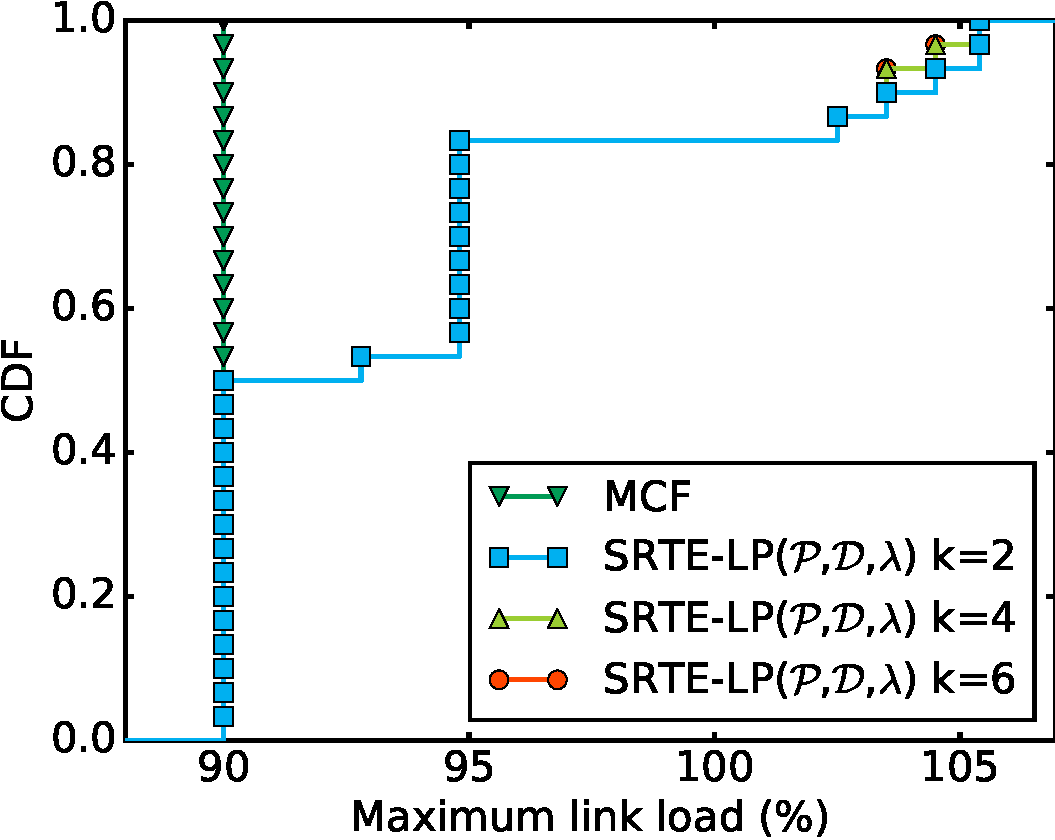
\includegraphics[width=0.8\textwidth]{images/solver_lower_bound_seg_cmp.2016RocketFuelUCL.cdfs.pdf}
\end{center}
\caption{Lower bound}
\label{fig:optimum_lowerbound}
\end{figure}


%The first question to answer is how near \name~really is to the optimality.
\textbf{CG4SR provides solutions whose maximum load is at most 4\% more than the optimal solution.} 
We ran \name~without enabling adjacency segments and without time limit.
The experiment was repeated with limits of 2, 4 and 6 segments
to observe the impact of the segment limit on the quality of the solution.
Figure \ref{fig:optimum:gap} shows CDFs of the gap (in percents)
between the \name~upper and lower bounds
on all the 30 instances (i.e., 5 demand matrices for each of the 6 topologies)
and increasing the limit on the number of segments.
This gap is the maximum distance to the actual optimum.
We can see that increasing the limit from 2 to 4 segments impacts
the quality of the solution while increasing the limit from 4 to 6 has little impact.
Paths with 4 or 6 segments add more flexibility than paths with 2 segments
to SRTE-UTIL-ILP.
We can see that this gap is most of the time below 1\% of the load and at worst 4\% of the load
if 4 segments are allowed.


\begin{figure}
\begin{center}
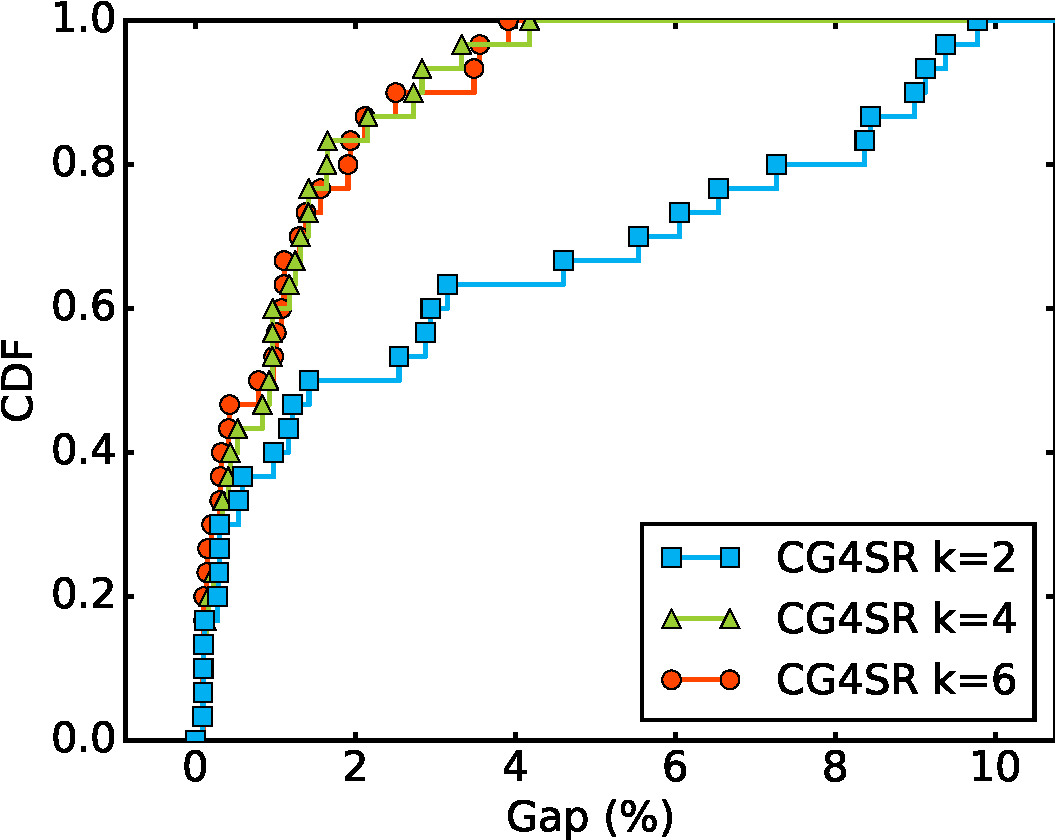
\includegraphics[width=0.8\textwidth]{images/solver_gap_optim_seg_cmp.2016RocketFuelUCL.cdfs.pdf}
\end{center}
\caption{Gap}
\label{fig:optimum:gap}
\end{figure}


\textbf{CG4SR is more efficient than Bhatia and MCF.} 
We compared the speed of \name~to Bhatia, MCF and MCFP. MCFP is an efficient variant of MCF that is only able to
compute the optimal value of MCF, not the actual routing paths.
%All these solvers provide guarantee on their final solutions.
Figure \ref{fig:optimum:time} describes how fast the different solvers can find
their best solution.
During these runs, the limit on the number of generated paths
at each column generation iteration, \textit{maxp} in Algorithm \ref{algo:iterate}, is fixed to 10.
This figure shows a CDF of the execution time on the different topologies and
demand matrices for \name, Bhatia and MCF.
Because Bhatia only allows two segments, \name~is also limited to two segments in this figure.
MCF is the slowest one and it runs out of memory for all the demand matrices
of the largest topology despite the 120GB available.
Bhatia only considers paths that can be expressed with two segments.
This significantly reduces the problem size and Bhatia can always get an answer.
\name~can run with any number of two segments because of the lazy generation of the paths.
And this is so effective than we are actually faster than Bhatia with a two-segment limit.

Figure \ref{fig:optimum:time} also shows that the MCFP variant of MCF
can actually compute the optimal value of the MCF quicker than \name.
But, as mentioned above, MCFP only provides the maximum link
utilisation of the MCF formulation but not a set of paths satisfying it. Hence, in practice, MCFP can
only be used to provide lower bounds which, as we showed in Figure \ref{fig:optimum:gap}, are worse
than the ones provided by our algorithm.

%while the optimal value is the same as the MCF formulation,
%we cannot extract paths that satisfy its optimal value.
%Moreover,there is no guarantee that the MCFP solution is actually reachable,
%nor how far from the real optimal it could be.

\begin{figure}
\begin{center}
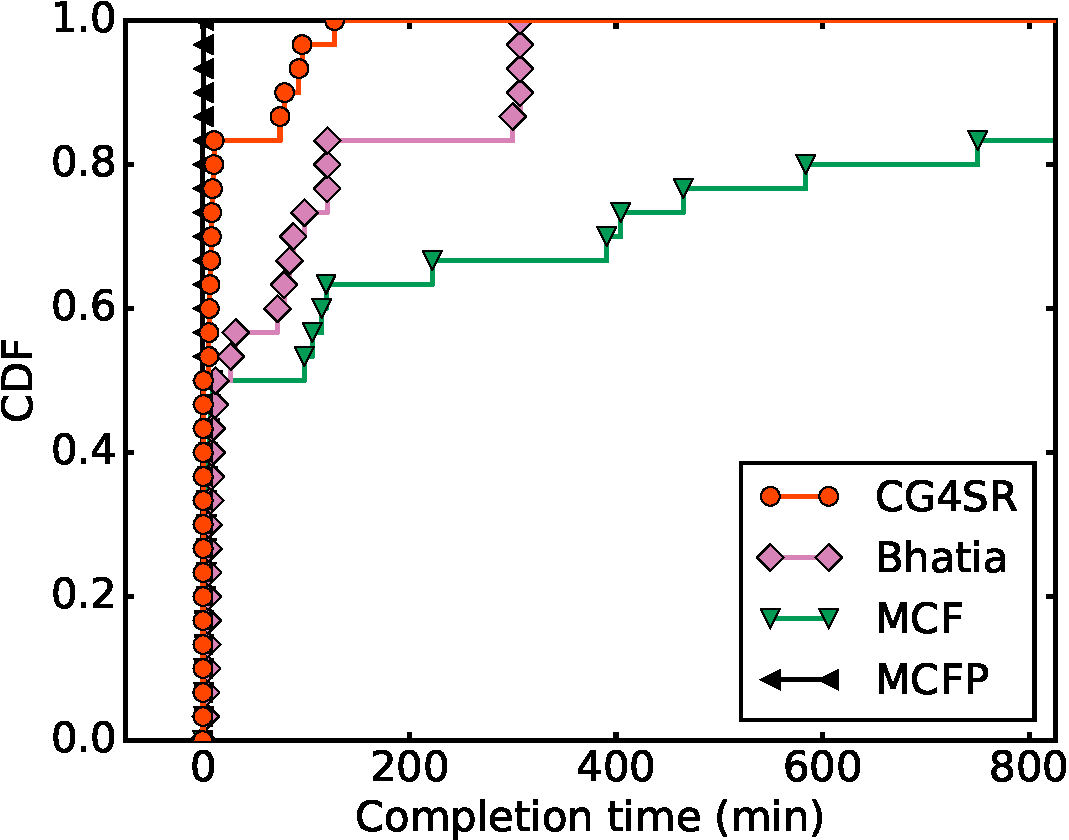
\includegraphics[width=0.8\textwidth]{images/solver_exec_times_inf-2.2016RocketFuelUCL.cdfs.pdf}
\end{center}
\caption{Execution time (\name~is limited to two segments)}
\label{fig:optimum:time}
\end{figure}


\textbf{CG4SR scales better than MCF and Bhatia.}
Our model has fewer variables than the MCF and Bhatia formulations.
The size of our model is the number of paths that were generated.
The size of MCF considers how much of each demand can be placed on each edge.
Therefore, the number of variables is the number of edges multiplied by the number of demands.
Bhatia considers for each demand, two segments through a single node of the graph.
Its number of variables is thus the number of nodes multiplied by the number of demands.
We observe that \name~is more scalable
because it considers at worst 60 times fewer possibilities than Bhatia
and 200 times fewer than MCF. This explains why \name~is faster than Bhatia and MCF.
This difference does not change significantly when varying the limit on the number of segments.
As can be seen in Figure \ref{fig:size:colgen},
the number of generated columns seems to grow linearly with the number of demands.
Given that the restricted path set is initialized with all the direct paths for every demand,
the path-finding process (Algo \ref{algo:iterate}) only creates a limited number
of additional paths to reach optimality.
This also explains why the column generation approach is so efficient in practice, as it only needs to solve the linear program
with a number of variables only slightly above the number of demands.
%\todo{Pierre: Enough dots for conclusions ?}

\begin{figure}
	\centering
	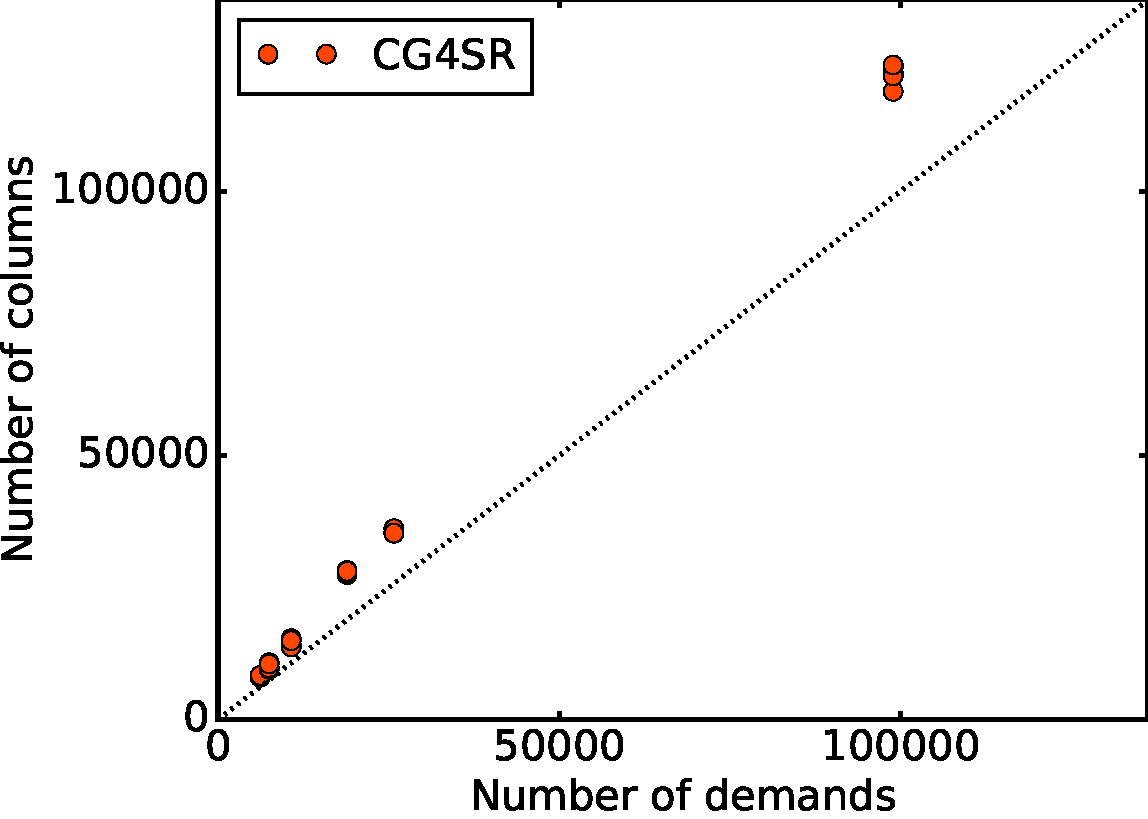
\includegraphics[width=0.8\textwidth]{images/solver_columns_over_demands_inf-6.2016RocketFuelUCL.pdf}
	\caption{Number of generated columns over the size of the demand matrices}
	\label{fig:size:colgen}
\end{figure}


\subsection{Any-time behavior}

The previous section shows that we can produce quality solutions with illimited time budget.
This section evaluates the quality of \name~solutions over time.
We compare \name~ to the heuristic approaches DEFO, SRLS and also to Bhatia.

\textbf{CG4SR finds good solution even if only allowed to run for a short amout of time.}
Figures \ref{fig:anytime:1min}, \ref{fig:anytime:5min}
and \ref{fig:anytime:10min} show, for each of the cited solvers, a CDF of the gap
to the SRTE-LP solution for the cited solvers after,
respectively 1 minute, 5 minutes and 10 minutes.
During these runs, the \textit{maxp} parameter (see Algorithm \ref{algo:iterate}) of \name, is fixed to 10.
The limit of segments is set to 5, except for Bhatia which limits itself to 1.
The quality of a solution is the difference between its current solution and the \name~lower bound
that was computed without time limit and the same limit on the number of segments.

We see that we are always faster than Bhatia even with limited time spans.
SRLS and DEFO are heuristic approaches and therefore are able to quickly find good solutions.
Figure \ref{fig:anytime:1min} shows that \name~ is already comparable to SRLS and better than DEFO
for half of the instances after 1 minute.
We see that DEFO initially finds better solutions but \name~catches up for most of instances
by increasing the timeout in Figure \ref{fig:anytime:5min} and Figure \ref{fig:anytime:10min}.
The largest instance is not yet solved after 10 minutes and that explains why DEFO is still better.

\begin{figure}
\begin{center}
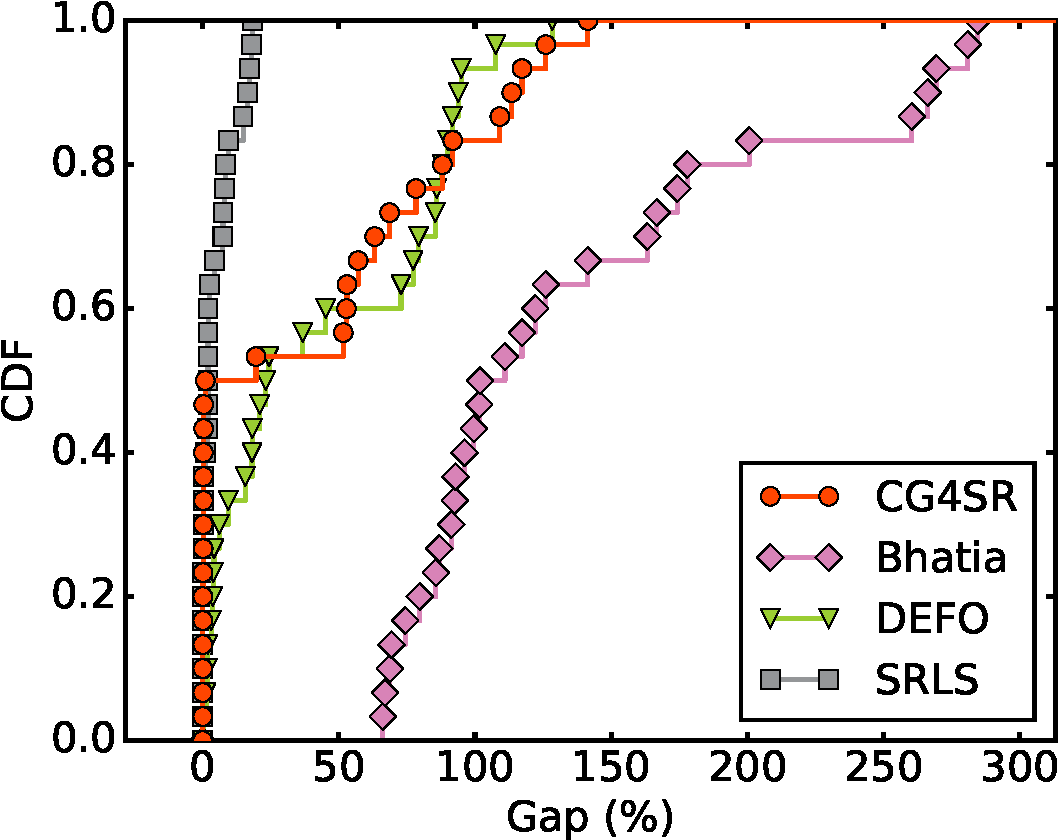
\includegraphics[width=0.8\textwidth]{images/solver_gap_optim_60-6.2016RocketFuelUCL.cdfs.pdf}
\caption{Timeout at 1 minute}
\label{fig:anytime:1min}
\end{center}
\end{figure}

\begin{figure}
\begin{center}
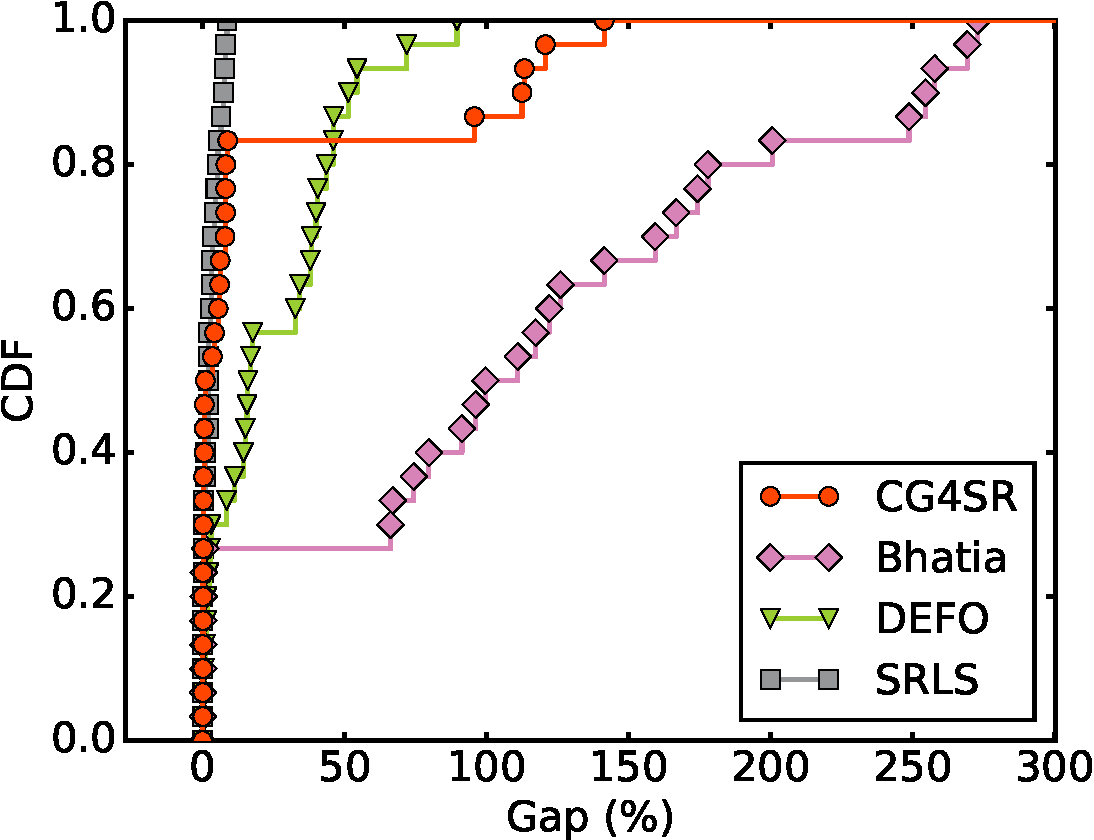
\includegraphics[width=0.8\textwidth]{images/solver_gap_optim_300-6.2016RocketFuelUCL.cdfs.pdf}
\caption{Timeout at 5 minutes}
\label{fig:anytime:5min}
\end{center}
\end{figure}

\begin{figure}
\begin{center}
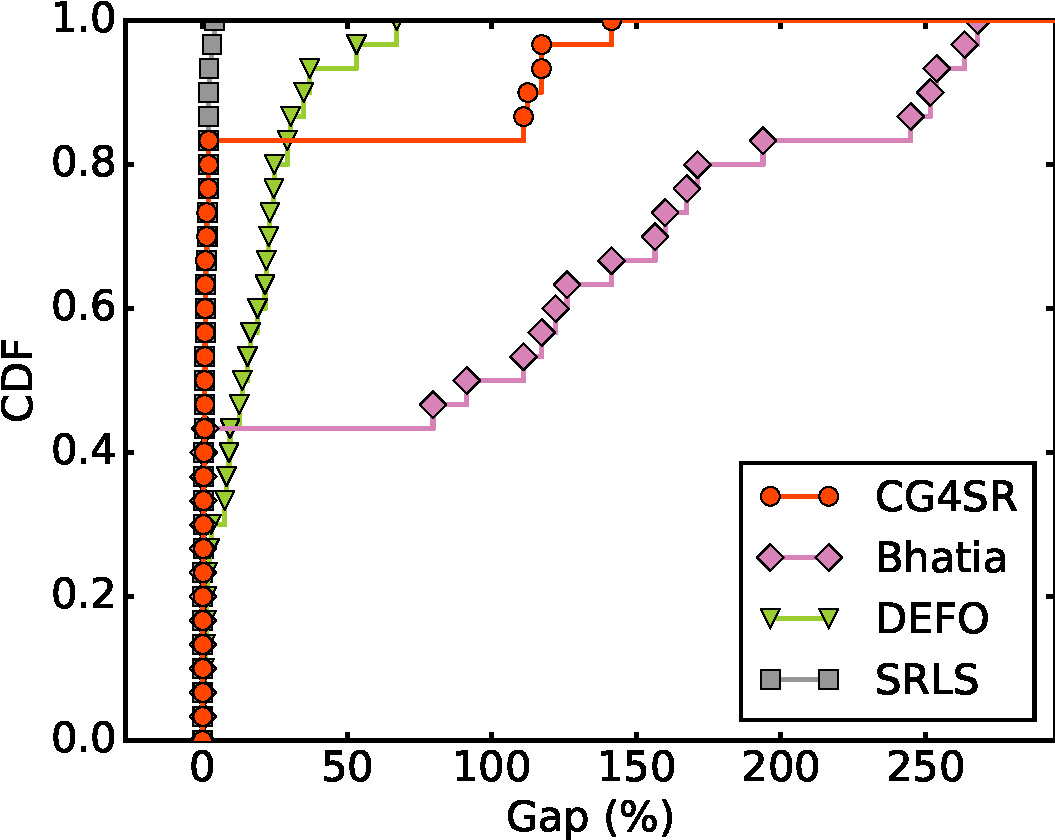
\includegraphics[width=0.8\textwidth]{images/solver_gap_optim_600-6.2016RocketFuelUCL.cdfs.pdf}
\caption{Timeout at 10 minutes}
\label{fig:anytime:10min}
\end{center}
\end{figure}


\textbf{CG4SR is more robust than SRTE over different sets of demands.}
SRLS produces good results but however this solution is based on local search and can be stuck in a local optimum.
We did not observe it on the demand matrices generated by the gravity model.
The demand volumes are generally much lower than link capacities.
This also means that there are many possible ways to reach good solutions,
even if the best solution is hard to find.
The gravity model is a good match to the Traffic Engineering problem in ISPs
but demand volumes are likely higher in inter-datacenter communication \cite{b4}.
This also means that there are fewer good solutions.
We generated one additional demand matrix for each RocketFuel topology
with a low number of large demands requiring 95\% of the bandwidth available
between their source and destination.
Figure \ref{fig:anytime:srlsdefense} shows a CDF of the quality of the solution with
a time limit of 10 minutes and a limit of six segments as in Figure \ref{fig:anytime:10min}.
These results confirm that SRLS can be worse than \name~when fewer good solutions are available.

\begin{figure}
	\centering
	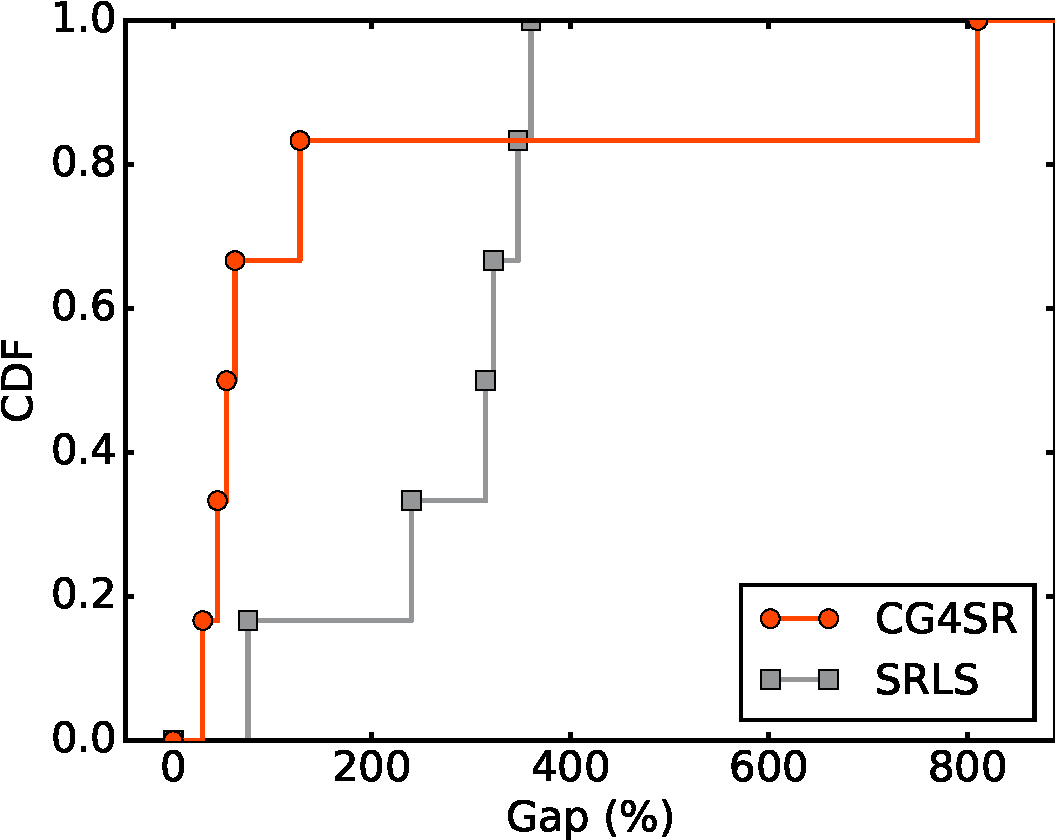
\includegraphics[width=0.8\textwidth]{images/solver_gap_optim_600-6.2016RocketFuelUCL_datacenter.cdfs.pdf}
	\caption{Gaps between $SRTE-LP(\P,\D,\lambda)$ and SRLS or \name~after 10 min with a limit of 6 segments}
	\label{fig:anytime:srlsdefense}
\end{figure}

%\textbf{CG4SR avoids to use SR on too many paths.}
%The gap is not the only criteria of the quality of a solution.
%Since the encoded stack of Segment Routing labels takes space into each packet,
%they take bandwidth resources to be transmitted.
%That is, if two solutions have the same gap to \name~lower bound,
%it's best to choose the one with fewer paths with at least two segments.
%Figure \ref{fig:anytime:10min:detours} shows how many paths need at least two segments to reach the solutions
%in Figure \ref{fig:anytime:10min}.
%We see that Bhatia finds solutions mostly without any segment but they have bad gaps,
%meaning that Bhatia did not have the time to find segments.
%When its gaps are good, it uses 2 segments on almost all the paths.
%\name~cannot find good segments for 5 instances (the demand matrices of the largest topology).
%Yet, for all the other instances, for a similar gap, it detours fewer demands than SRLS.
%DEFO detours fewer paths than \name~ but cannot always reach similar gaps.

%\begin{figure}
%	\centering
%	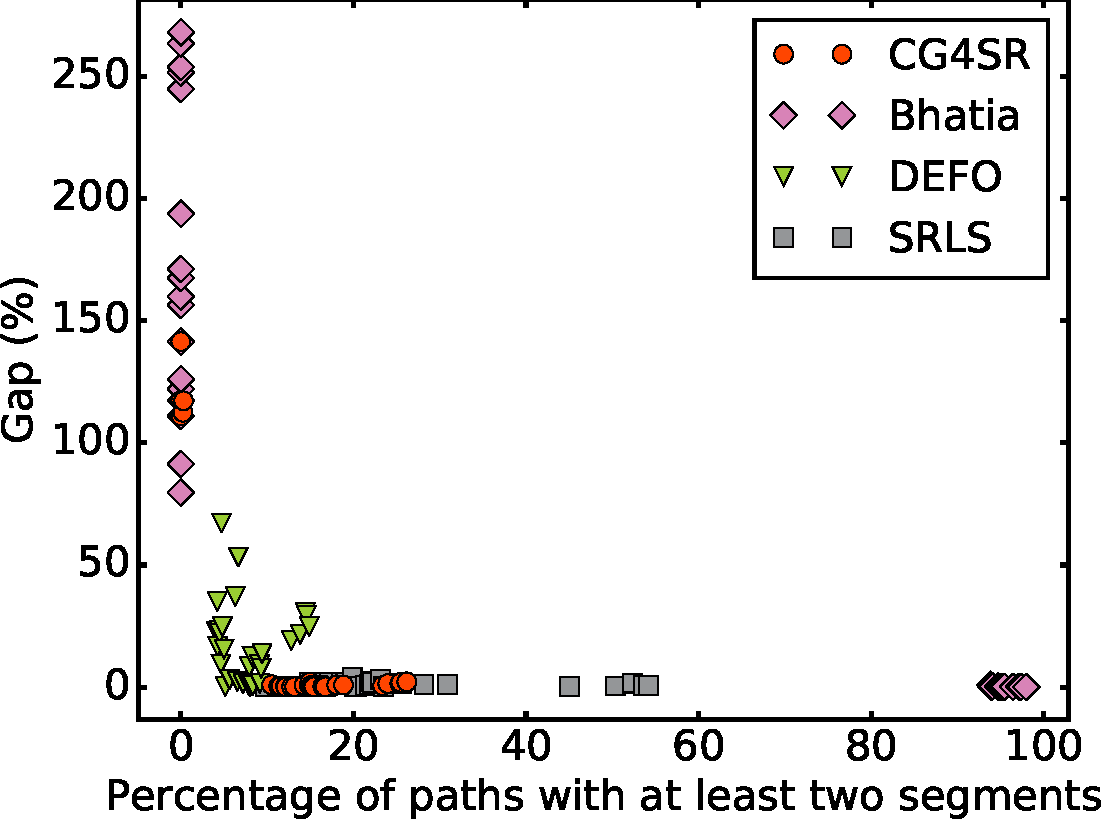
\includegraphics[width=0.3\textwidth]{images/solver_detoured_paths_600-6.2016RocketFuelUCL.pareto.pdf}
%	\caption{Gaps over the percentage of paths with at least two segments. We fixed the time limit to 10 minutes and the limit of segments to 6.}
%	\label{fig:anytime:10min:detours}
%\end{figure}

\subsection{Adjacency segment benefits}

\textbf{Adjacency segments are important in TE and CG4SR is the first to use them.}
\name~is the first SR traffic engineering model to support adjacency segments.
We evaluate the benefits of adjacency segments on the inter-datacenter network topology of OVH
in Europe (described in \cite{scmon}).
This topology has more parallel links than RocketFuel topologies and
thus, the OVH topology can really benefit from adjacency segments.
We do not have access to the link weights and capacities of OVH.
Therefore, for each link bundle we set the capacity of half of the links to some value and the other
half to half of that value. This simulates the link upgrades on the network. For pairs of
nodes with a single link between them, we set the capacity to be ten times bigger.
Five demand matrices were generated for the OVH topology with the gravity model \cite{gravitymodel}.

Figure \ref{fig:adjacency:upperbound} shows CDFs of the gap (in percents)
between the \name~upper and lower bounds over the demand matrices of the OVH topology.
We do not limit the execution time and we limit the number of segments to 4.
This means that we allow at most one detour through a specific link
because one segment is needed for the destination and a link detour costs two segments.
Even allowing only one link detour halves the load of the maximally loaded link
because it utilizes better the parallel links of this topology.

\begin{figure}
	\centering
	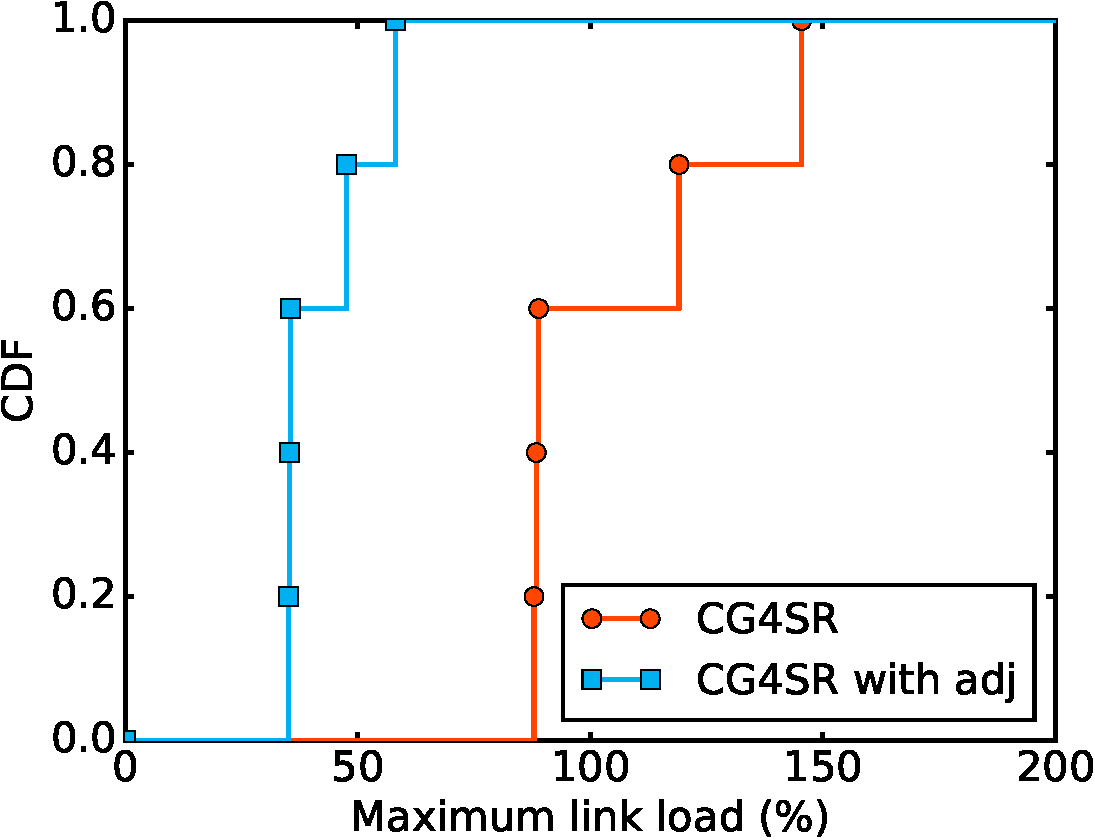
\includegraphics[width=0.8\textwidth]{images/solver_adj_upper_bound.OVH_paper.cdfs.pdf}
	\caption{The \name~solutions with or without adjacency segments. The limit of segments is fixed to 4.}
	\label{fig:adjacency:upperbound}
\end{figure}



\section*{Conclusion}

In this chapter we propose                                                                                                                                                                                                                                                                                                                                                                                                                   the first solution to exploit column generation to solve segment routing problems.
We believe that column generation is a good approach for solving segment routing problem and reinforce this
belief in the next chapter. The structure of sr-paths make it amiable to dynamic programming algorithms so
we feel that it will often be the case that the pricing problem will have a nice DP optimal substructure.

Our solution improves the state of the art lower bound making it possible to better evaluate the quality
of heuristic solutions. We also showed that even tough we are slower on demands generated according to a 
gravity model, with more constrained demands we can actually be much more efficient than local search.

It still remains an open problem to find an algorithm capable of providing optimal solution to the TE problem 
over segment routing within reasonable amount of time. We are unsure whether wrapping our solution with a branch-and-price
is the right way to go but it is certainly an interesting possibility.
